%
% Author:  Klára Pacalová
% E-mail:  pacalkla@fel.cvut.cz
% Date:    24.02.2018 11:03
%
\documentclass[twoside]{article}
\usepackage[a4paper]{geometry}
\geometry{verbose,tmargin=2.5cm,bmargin=2cm,lmargin=2cm,rmargin=2cm}
\usepackage{fancyhdr}
\pagestyle{fancy}
\usepackage[utf8]{inputenc}
\usepackage[czech]{babel}
\usepackage{siunitx}
\usepackage{listings}
\usepackage{graphicx} %graphics files inclusion
\usepackage{amsmath} %advanced maths
\usepackage{amssymb} %additional math symbols
% nastavení pisma a češtiny
\usepackage{lmodern}
\usepackage[T1]{fontenc}
\usepackage{float}

% odkazy
\usepackage{url}

% vícesloupcové tabulky
\usepackage{multirow}
\usepackage{listings}

% vnořené popisky obrázků
\usepackage{subcaption}

% automatická konverze EPS 
\usepackage{graphicx} 
\usepackage{epstopdf}

% odkazy a záložky
\usepackage[unicode=true, bookmarks=true,bookmarksnumbered=true,
bookmarksopen=false, breaklinks=false,pdfborder={0 0 0},
pdfpagemode=UseNone,backref=false,colorlinks=true] {hyperref}

% Poznámky při překladu
\usepackage{xkeyval}	% Inline todonotes
\usepackage[textsize = footnotesize]{todonotes}
\presetkeys{todonotes}{inline}{}

% Zacni sekci slovem ukol

% enumerate zacina s pismenem
\renewcommand{\theenumi}{\alph{enumi}}

% smaz aktualni page layout
\fancyhf{}
% zahlavi
\usepackage{titling}
\fancyhf[HC]{\thetitle}
\fancyhf[HLE,HRO]{\theauthor}
\fancyhf[HRE,HLO]{\today}
 %zapati
\fancyhf[FLE,FRO]{\thepage}

% údaje o autorovi
\title{Analogový přeladitelný filtr se zesilovači OTA}
\author{Klára Pacalová}
\date{\today}

\begin{document}
\definecolor{MapleBlue}{rgb}{0,0,1}
\def\MapleOutput#1{{\begin{center}\begin{math}\color{MapleBlue}{#1}\end{math}\end{center}}}

\maketitle

% ---------------------------------
% ---------------------------------
% název sekce je generován automaticky jako: Úkol X
Klíčová slova: \textit{transkonduktance, OTA, OTA-C, analogový filtr, pásmová propust, dolní propust}
\section{Motivace}
\noindent Cílem práce je navrhout zapojení analogového filtru typu pásmová propust 4. řádu s OTA. Hlavním nástrojem je Maple s knihovnou Syntfil, obvodová simulace je poté realizována v prostředí Multisim.
\section{Analogové filtry}
Filtry jsou určeny k potlačení nebo zvýraznění určité části kmitočtového spektra signálu. Jsou to obvody s kmitočtově závislou přenosovou funkcí (pro napěťový přenos $H_s(j \omega) = \frac{U_{out}(j \omega)}{U_{in}(j \omega)}$). Základní rozdělení je na dolní propust (\textit{low-pass} - LP), horní propust(\textit{high-pass} - HP), pásmovou propust (\textit{band-pass} - BP) a pásmovou zádrž (\textit{band-stop} - BS). \\
\\
Dolní propust nepropouští na výstup vstupní signál nad frekvencí $f_s$, signál v propustném pásmu zůstává beze změny nebo zesílený. Základní pasivní dvojbranné zapojení je ke vstupu sériově zapojený rezistor a k této větvi paralelně kapacitor. Tento RC člen se zvyšující se frekvencí snižuje svou vstupní impedanci. Přenosová funkce má nulu v nekonečnu a pól v levé polorovině s-roviny. Ideální integrátor má pól v nule. \\
Horní propust nepropouští signály o nízkých frekvencích. Nejjednodušší zapojení je RC člen, kdy kapacitor je zapojen sériově se zdrojem a k této větvi paralelně rezistor. Pro toto zapojení reaktance kapacitoru se zvyšující se frekvencí klesá. Přenosová funkce ideálního derivátoru má pól v nekonečnu a nulu v nule. Horní propust má nulu v nule a pól v levé polorovině s-roviny.\\
\\
Pásmová propust propouští pásmo určené dvěma kmitočty. Pasivní pásmové propusti nedosahují účinnosti větší než 1. Jsou složeny z integračního článku (RC - dolní propust) a derivačního článku (CR - horní propust).\\
\\
Pásmová zádrž nepropouští kmitočty pásma definovaného dvěma kmitočty. Pasivní zapojení je složeno ze dvou rezistorů a kapacitorů. Má vždy ztrátový přenos.
\begin{figure}[H]
\centering
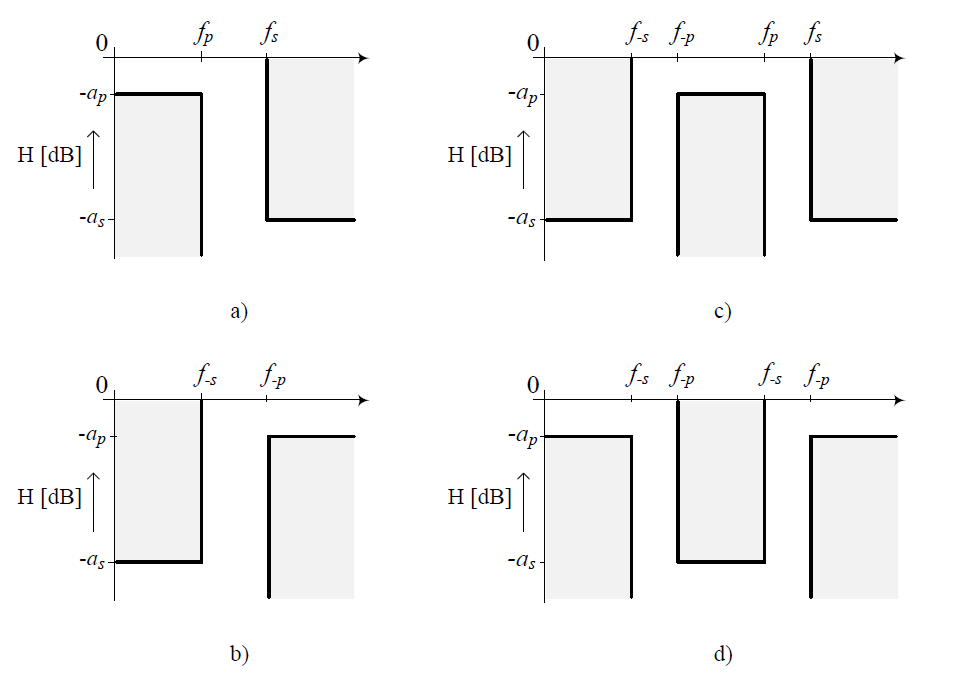
\includegraphics[scale=0.55]{tolerancnischemata.png}
\caption{Toleranční schéma pro a) dolní propust (LP), b) horní propust (HP), c) pásmovou propust (BP) a d) pásmovou zádrž (BS)\cite{1}}
\end{figure}
\noindent Filtry se používají k redukci nežádoucích frekvencí např. pro efektivní reprodukci zvuku reproduktory, k redkci okolního rušení např. vysílače blokují harmonické frekvence, které interferují, jako filtry v obvodech rekonstrukce signálů u D/A převodníků, nebo jako anti-aliasing filtry např předvzorkování u A/D převodníku).\\\\
Obecná přenosová funkce filtru typu dolní propust je
\begin{align}
H(j\omega) = \frac{H_0}{\prod_{i=1}^{\frac{n}{2}} (1 + a_i s + b_i s^2)},
\end{align}
kde $n$ je řád filtru.\\
Obecná přenosová funkce filtru typu horní propust je
\begin{align}
H(j\omega) = \frac{H_{\infty}}{\prod_{i=1}^{\frac{n}{2}} (1 + \frac{a_i}{s} + \frac{b_i}{s^2})},
\end{align}
kde $n$ je řád filtru.\\
Podle rozložení nul a pólů jmenovatele rozlišujeme různé aproximace. Koeficienty filtru $a_i, b_i$ určují zesílení v propustném pásmu. Činitel jakosti je definován jako $Q = \frac{\sqrt{b_i}}{a_i}$. Čím větší $Q$ je obdrženo, tím spíš bude filtr nestabilní.
\begin{figure}[H]
\centering
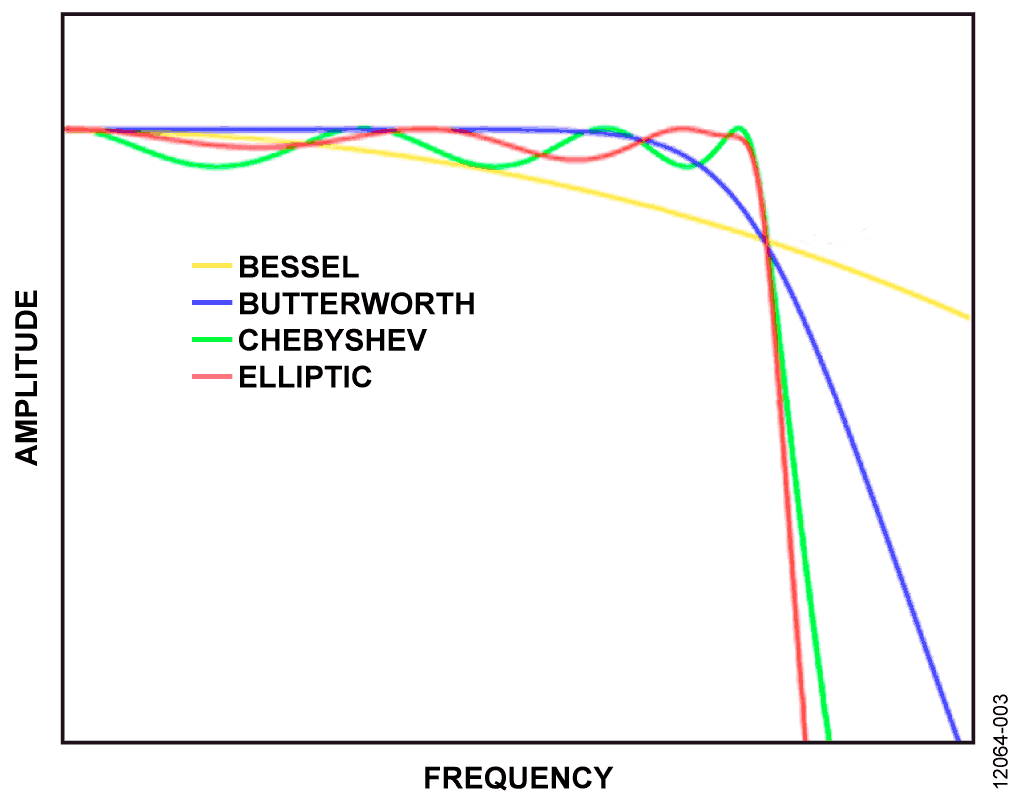
\includegraphics[scale=0.3]{LGA98.png}
\caption{Typy aproximací (LP)\cite{2}}
\end{figure}
\subsection{Butterworthova aproximace}
Butterworthova má maximálně plochou amplitudovou charakteristiku v propustném pásmu. Frekvenční charakteristika má sklon daný počtem pólů a pro její posouzení je užíváno skupinové zpoždění (derivace fáze podle frekvence). Pro Butterworthovu aproximaci je skupinové zpoždění nezvlněné v propustném pásmu. Přechodová charakteristika má mírný překmit, zvyšující se s řádem filtru. Zesílení $G(\omega)$ je kmitočtově závislé a odpovídá absolutní hodnotě přenosové funkce $H(j\omega)$.
\begin{align}
G(\omega) = |H(j\omega)| = \frac{1}{\sqrt{1 + \epsilon ^2 \frac{\omega}{\omega _c}^{2n}}},
\end{align}
kde $\epsilon$ je poměrné zvlnění kmitočtové charakteristiky v propustném pásmu (\textit{faktor zvlnění}), $n$ je řád filtru a $\omega _c$ mezní frekvence. Mezní frekvence je definována jako frekvence, která nastává při útlumu -3 dB. Pro $\omega _c = 1$ je faktor zvlnění $\epsilon = 1$. 
\subsection{Čebyševova aproximace}
Čebyševova aproximace má strmější pokles, což vede k užití nižšího řádu filtru. Zato má ale zvlněnou frekvenční charakteristiku v propustném pásmu. 
\subsubsection{Typ I}
Vyjádření modulové charakteristiky pro tuto aproximaci je dáno jako
\begin{align}
G(\omega) = |H(j\omega)| = \frac{1}{\sqrt{1 + \epsilon ^2 T_n ^2 \frac{\omega}{\omega _c}^{2n}}},
\end{align}
kde $T_n$ je Čebyševův polynom, $\epsilon$ je poměrné zvlnění, $n$ je řád filtru a $\omega _c$ mezní frekvence. Čebyševův polynom je definován vztahem $2 \omega ^2 - 1$ pro $n = 2$. Obecně jsou to kořeny Chebyshevových diferenciálních rovnic
\begin{align}
(1 - x^2)y" - xy' + n^2y = 0\\
(1 - x^2)y" - 3xy' + n(n+2)y = 0.
\end{align}
\subsubsection{Typ II}
Typ II je nazýván také jako inverzní Čebeševova aproximace. V praxi není příliš používaný, jelikož nemá tak rychlý pokles jako typ I a k jeho realizaci je třeba více prvků. Nemá zvlnění v propustném pásmu, zato v zádržném ano. Zesílení je definováno jako
\begin{align}
G(\omega, \omega _c) = \frac{1}{\sqrt{1 + \frac{1}{\epsilon ^2 T_n ^2 \frac{\omega _c}{\omega}^{2n}}}},
\end{align}
kde $T_n$ je Čebyševův polynom, $\epsilon$ je poměrné zvlnění, $n$ je řád filtru a $\omega _c$ mezní frekvence.
\subsection{Besselova aproximace}
Besselova aproximace se používá v telekomunikační technice v případech, kdy je požadováno zachování tvaru signálu. Amplitudová charakteristika v nepropustném pásmu je velmi plochá. Koeficienty polynomu jsou zvoleny tak, aby fázová charakteristika v pásmu okolo kritické frekvence byla maximálně lineární. Nevýhodou je poměrně malá strmost modulové charakteristiky. Ta je pro Besselovu aproximaci je dána vztahem
\begin{align}
G(\omega) = |H(j\omega)| = \frac{\Theta _n(0)}{\Theta _n(\frac{j\omega}{\omega _c})},
\end{align}
kde $\Phi _n$ je Besselův polynom a $\omega _c$ mezní frekvence. Besselův polynom je definován součtem řady (Grosswald 1978, Berg 2000)
\begin{align}
\Theta _n (x) = x^n y_n (\frac{1}{x}) = \sum_{k=0}^{n}\frac{(n+k)!}{(n-k)!k!}\frac{x^{n-k}}{2^k}.
\end{align}
Pro filtr druhého řádu platí
\begin{align}
G(\omega) = |H(j\omega)| = \frac{3}{\sqrt{\omega ^4 + 3\omega ^2 + 9}}.
\end{align}
\subsection{Cauerova (eliptická) aproximace}
\noindent Cauerova aproximace (eliptická) má nejstrmější pokles, při jejím užití jsou voleny nižší řády filtru. Pokud se zvlnění v zádržném pásmu blíží nule, filtr se stává Čebyševovým (výše zmíněný - typ I). Opačně je tomu v propustném pásmu - přiblížením k nule se filtr stává inverzním Čebyševovým (typ II).  Pokud se obě hodnoty zvlnění blíží k nule, filtr se stává Butterworthovým. Kmitočtová charakteristika je dána vztahem
\begin{align}
G(\omega) = |H(j\omega)| = \frac{1}{\sqrt{1 + \epsilon ^2 R_n ^2(\zeta, \frac{\omega}{\omega _c})}},
\end{align}
kde $\epsilon$ je faktor zvlnění, $R_n$ eliptická racionální funkce n-tého řádu, $\zeta$ selektivní faktor a $\omega _c$ mezní frekvence. Pokud pro selektivní faktor platí $\zeta \rightarrow \infty$, filtr se stává Čebyševovým (typ I). 
\section{Transkonduktanční zesilovače (OTA)}
V telekomunikacích se používají filtry v rozsahu kmitočtů desítek až stovek megahertz, v bezdrátové komunikaci až v řádu gigahertz. Běžné RC filtry by neměly být užívány ve frekvenčním rozsahu nad 5-10$\%$ $\omega _c$ - tedy v tomto rozsahu používaném v telekomunikačních technologiích nemají předvídatelné průběhy. Krom toho ve spínačích CMOS, kde rezistory běžně nejsou dostupné, jsou potřeba zesilovače s velkou šířkou pásma a zároveň vysokým zesílením. Dodržení těchto požadavků je náročné a drahé. Dalším extrémem pro analogové integrované filtry jsou telefonní linky, kde jsou kmitočtové rozsahy sice nízké, ale je požadována nízká cena a vysoká přesnost.\\
\\
Pro nízké frekvence se ke splnění těchto požadavků používají obvody se spínanými kapacitory (SC). Přepínaný kapacitor se chová jako rezistor, tudíž časová konstanta RC je definována poměrem kapacitorů a hodinovou (CLK) frekvencí, se kterou jsou přepínány. Pro vysokofrekvenční aplikace (až v řádu gigahertz) se používají MOSFET-C filtry.\\
\\
Další z možných prvků, které jsou dostupné jak pro nízkofrekvenční aplikace, tak pro kmitočtový rozsah stovek megahertz, jsou transkonduktanční zesilovače.\\\\
Transkonduktanční zesilovače (označují se též jako OTA (\textit{Operational Transconductance Amplifiers}) jsou napětím řízené zesilovače s proudovým výstupem - zdroje proudu
\begin{align}
i_{out} = g_m(u_+ - u_-),
\end{align}
kde $u_+$ a $u_-$ jsou napětí invertujícího a neinvertujícího vstupu.  Transkonduktance je řízena externím proudem $I_{ABC}$ (\textit{Bias Current}). Ideální OTA má kmitočtově nezávislou transkonduktanci $g_m$ (na rozdíl od reálného, který je kmitočtově závislý).
\begin{figure}[H]
\centering
\includegraphics[scale=0.7]{image7.png}
\caption{OTA - schematické značky \cite{3}}
\end{figure}
\begin{figure}[H]
\centering
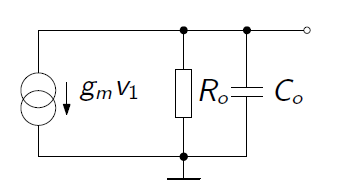
\includegraphics[scale=0.6]{gmrc.png}
\caption{Linearizovaný model reálného OTA \cite{4}}
\end{figure}
\noindent Připojením zátěže $R_z$ na výstup bylo získáno napětí naprázdno
\begin{align}
u_{out} = R_zg_m(u_+ - u_-) = G_0(u_+ - u_-),
\end{align}
kde $G_0$ je zesílení. Ze vztahu (2) plyne, že zesílení je konečné a mezi vstupy je nenulové napětí. Připojením kondenzátoru jako zátěže byl získán bezeztrátový integrátor s přenosem
\begin{align}
H(s) &= \frac{v_2}{v_1} = \frac{g_m}{sC} \\
v_0(t) &= \frac{1}{C}\int i(t)dt = \frac{1}{C}\int g_mv_1(t)dt.
\end{align}
\begin{figure}[H]
\centering
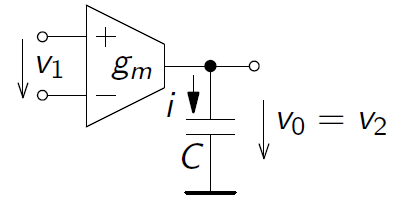
\includegraphics[scale=0.5]{otaintegrator.png}
\caption{OTA-C \cite{4}}
\end{figure}
\noindent Toto zapojení integrátoru s uzemněným kondenzátorem se označuje jako OTA-C.\\
\\
Ztrátový integrátor lze utvořit sériovým zapojením dalšího OTA jako odporu se zápornou zpětnou vazbou. Rozdíl mezi ideálním a ztrátovým integrátorem lze pozorovat i v modulové charakteristice - pro ztrátový je konstantní a pak teprve lineárně klesá se sklonem -20 dB/dek.
\begin{align}
v_0(t) = \frac{g_{m1}}{sC + g_{m2}}(v_1^+ - v_{1}^-)
\end{align}
\begin{figure}[H]
\centering
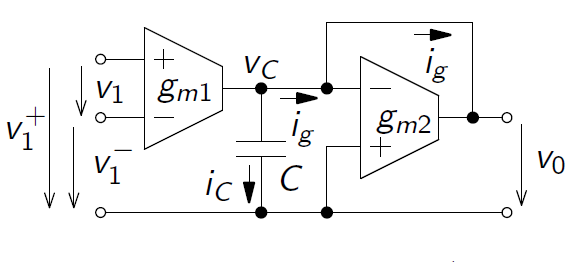
\includegraphics[scale=0.5]{damp.png}
\caption{Ztrátový OTA-C \cite{4}}
\end{figure}
\section{Integrované obvody s OTA}
Integrované obvody se vyrábí buď s jedním nebo dvěma zesilovači v pouzdře. Varianty s jedním operačním zesilovačem jsou např. OPA615, OPA860 a novější OPA861. Všechny součástky s jedním OZ mají velkou šířku pásma (v řádech stovek MHz), cenově vychází na 75-280 Kč. Integrované obvody s dvěma OZ v pouzdře mají užší šířku pásma (2 MHz), menší rychlost přeběhu (50 V/$\mu$s), mnohem menší výstupní proud (650 $\mu$A) i offset vstupního napětí a operují při cca 4x nižších proudech. Cenové rozpětí je 25-65 Kč.
\renewcommand{\arraystretch}{1.5}
\begin{table}[H]
\scalebox{0.9}{%
  \begin{tabular}{ | c | >{\centering\arraybackslash}p{2cm}| >{\centering\arraybackslash}p{1.5cm} | >{\centering\arraybackslash}p{1.5cm} | >{\centering\arraybackslash}p{1.25cm} | >{\centering\arraybackslash}p{1.5cm} | >{\centering\arraybackslash}p{1.75cm} | >{\centering\arraybackslash}p{2cm} | >{\centering\arraybackslash}p{1.75cm} |}
    \hline
      & GBP - Gain Bandwidth Product & SR - Slew Rate & Output Current per Channel & $I_b$ - Input Bias Current & $V_{os}$ - Input Offset Voltage & Operating Supply Current & Forward Transconductance Min & Supply Voltage\\ \hline
    OPA615 & 710 MHz & 2.5 kV/$\mu$s & 5 mA & 3 $\mu$A & 40 mV & 13 mA & 65 mA/V & 8-12.4 V \\ \hline
    OPA860 & 470 MHz & 3.5 kV/$\mu$s & 15 mA & 5 $\mu$A & 12 mV & 11.2 mA & 80 mA/V & 5-13 V \\ \hline
    OPA861 & 400 MHz & 900 V/$\mu$s & 15 mA & 1 $\mu$A & 12 mV & 5.4 mA & 65 mA/V & 4-12.6 V  \\
    \hline
  \end{tabular}}
  \caption{\label{tab:Porovnání integrovaných obvodů s jedním OTA}orovnání integrovaných obvodů s jedním OTA \cite{5}}
  \end{table}
\begin{center}
\begin{table}[H]
\scalebox{0.9}{%
  \begin{tabular}{ | c | >{\centering\arraybackslash}p{2cm}| >{\centering\arraybackslash}p{1.5cm} | >{\centering\arraybackslash}p{1.5cm} | >{\centering\arraybackslash}p{1.25cm} | >{\centering\arraybackslash}p{1.5cm} | >{\centering\arraybackslash}p{1.75cm} | >{\centering\arraybackslash}p{2cm} | >{\centering\arraybackslash}p{1.75cm} |}
    \hline
      & GBP - Gain Bandwidth Product & SR  - Slew Rate & Output Current per Channel & $I_b$ - Input Bias Current & $V_{os}$ - Input Offset Voltage & Operating Supply Current & Forward Transconductance - Min & Supply Voltage\\ \hline
    LM13700 & 2 MHz & 50 V/$\mu$s & 650 $\mu$A & 5 $\mu$A & 4 mV & 1.3 mA & 6700 $\mu$S & 10-36 V \\ \hline
    NE5517 & 2 MHz & 50 V/$\mu$s & 650 $\mu$A & 5 $\mu$A & 5 mV & 2.6 mA & 5400 $\mu$S & 4-44 V \\ \hline
    AU5517 & 2 MHz & 50 V/$\mu$s & 650 $\mu$A & 5 $\mu$A & 5 mV & 2.6 mA & 5400 $\mu$S & 4-44 V  \\ \hline
    NJM13600 & 2 MHz & 50 V/$\mu$s & 650 $\mu$A & 5 $\mu$A & 5 mV & 2.6 mA & 6700 $\mu$S & 36 V  \\ \hline
    NJM13700 & 2 MHz & 50 V/$\mu$s & 650 $\mu$A & 5 $\mu$A & 4 mV & 2.6 mA & 6700 $\mu$S & 36 V  \\ \hline
  \end{tabular}}
  \caption{\label{tab:Porovnání integrovaných obvodů se dvěma OTA}Porovnání integrovaných obvodů se dvěma OTA \cite{5}}
  \end{table}
\end{center}
\noindent Pro realizaci přeladitelného filtru byl zvolen LM13700 s dvěma OZ.
\begin{figure}[H]
\centering
\includegraphics[scale=0.55]{image6.png}
\caption{Konfigurace pinů na LM13700M \cite{6}}
\end{figure}
\noindent Vnitřní zapojení LM13700 na obrázku 8 obsahuje symetrický rozdílový stupeň (tranzistory Q4, Q5), který je napájen řízeným zdrojem proudu s tranzistorem Q2. Dvojice diod a tranzistorů tvoří proudová zrcadla (\textit{Current Mirror}) - referenční proud tekoucí v jedné větvi obvodu se "zrcadlí" v jeho druhé větvi. Principiálně jsou to zdroje proudu řízené proudem. 
\begin{figure}[H]
\centering
\includegraphics[scale=0.75]{image5.png}
\caption{Vnitřní chéma OTA \cite{6}}
\end{figure}
\section{Odvození DP 2. řádu}
Náhradní obvod, ze kterého bude spočítána přenosová funkce pro přenos filtru druhého řádu, popisuje obrázek 9.
\begin{figure}[H]
\centering
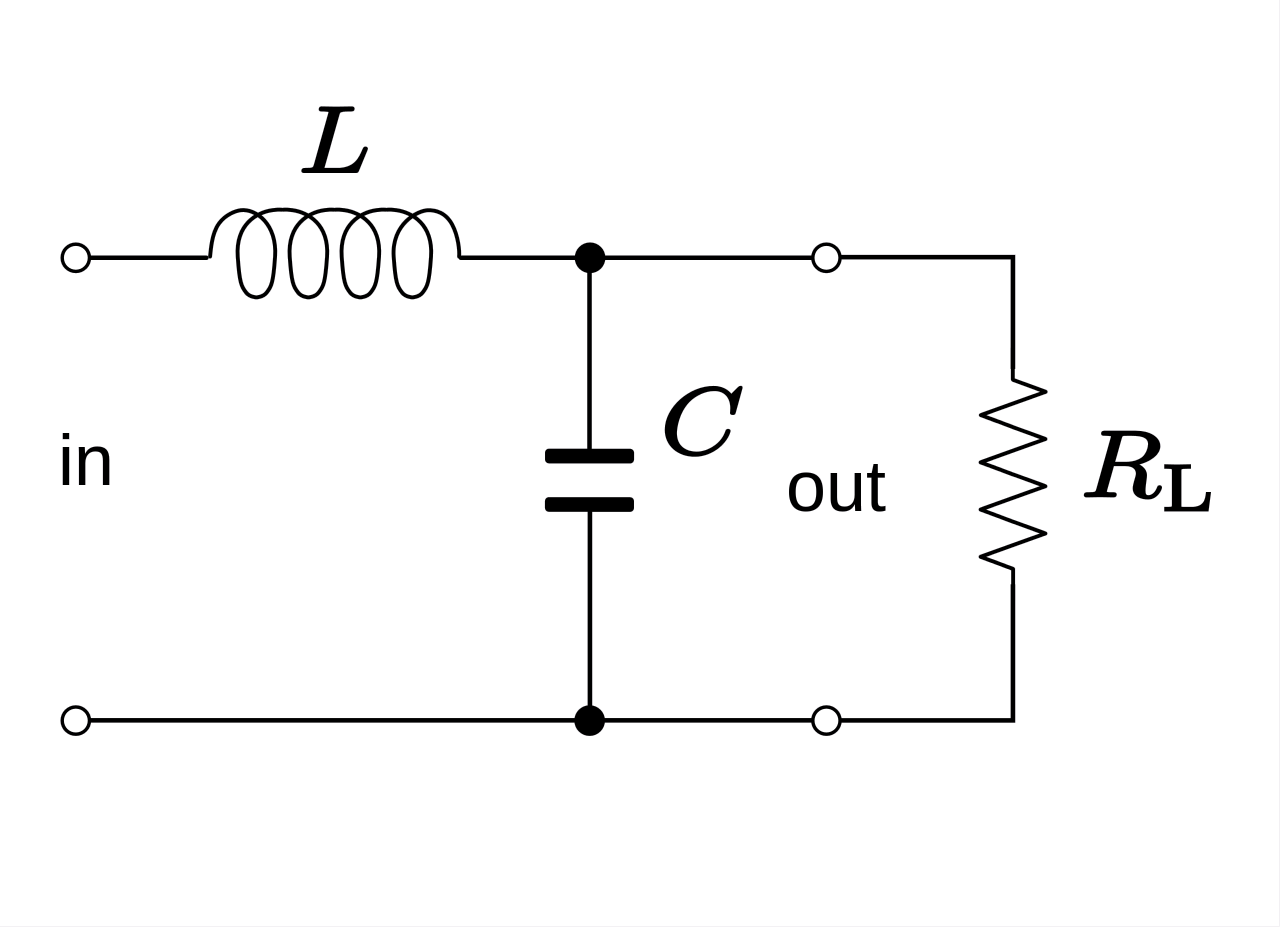
\includegraphics[scale=0.15]{RLC_low-pass.png}
\caption{Dolní propust 2. řádu \cite{7}}
\end{figure}
\noindent Přenos obvodu byl vyjádřen jako
\begin{align}
H(s) = \frac{U_{out}}{U_{in}} = \frac{Z_2}{Z_1},
\end{align}
kde $Z_1 = sL$ a $Z_2 = \frac{\frac{R}{sC}}{R + \frac{1}{sC}}$. Tedy
\begin{align}
H(s) = \frac{\frac{\frac{R}{sC}}{R + \frac{1}{sC}}}{sL + \frac{\frac{R}{sC}}{R + \frac{1}{sC}}}.
\end{align}
Elementárními algebraickými úpravami a následným vynásobením členem $\frac{1}{LRC}$ byl získán výsledný přenos.
\begin{align}
H(s) = \frac{R}{s^2LRC + sL + R} = \frac{\frac{1}{LC}}{s^2 + \frac{s}{RC} + \frac{1}{LC}}.
\end{align}
\noindent Pro ideální OTA zesilovač (vstupní i výstupní impedance nulové) je možno odpor nahradit obvodem s uzemněným neinvertujícím vstupem a zpětnou vazbou z invertujícího vstupu na výstup a to hodnotou
\begin{align}
R_{in} = \frac{1}{g_{m1}},
\end{align}
kde $g_{m1}$ označuje transkonduktanci zesilovače. Prohození invertujícího a neinvertujícího vstupu vede na opačnou polaritu.
\begin{figure}[H]
\centering
\includegraphics[scale=0.7]{image10.png}
\caption{Obvod pro simulaci uzemněného rezistoru \cite{8}}
\end{figure}
\noindent Pro nahrazení indukčnosti o impedanci $Z_L = \frac{1}{sC}$ lze použít obvod s třemi OTA. Uzemněny jsou invertující vstup prvního OTA a neinvertující druhého. Použita je zpětná vazba z výstupu na neinvertující vstup prvního OTA. Propojení výstupu prvního OTA na invertující vstup druhého OTA je realizován přes uzemněný kapacitor. \\
Vyjádřením napětí a proudů v obvodu bylo získáno napětí na kapacitoru a vstupní proud
\begin{align}
V_C &= \frac{g_{m1}}{sC}V_1 \\
I_1 &= g_{m2}V_C = \frac{g_{m1}g_{m2}}{sC}V_1.
\end{align}
Výsledná indukčnost - impedance vstupu byla vyjádřena vztahem (11).
\begin{align}
Z_{in}(s) = \frac{V_1}{I_1} = s\frac{C}{g_{m1}g_{m2}}
\end{align}
\noindent Byl obdržen induktor o hodnotě
\begin{align}
L = \frac{C}{g_{m1}g_{m2}}.
\end{align}
\begin{figure}[H]
\centering
\includegraphics[scale=0.55]{image13.png}
\caption{Obvod pro simulaci indukčnosti \cite{8}}
\end{figure}
\noindent Pro uzemněnou indukčnosti o impedanci $Z_L = \frac{1}{sC}$ byl použit obvod na obrázku 12. Vyjádřením napětí a proudů v obvodu bylo získáno napětí na kapacitoru a vstupní proud
\begin{align}
V_C &= \frac{g_{m1}}{sC}V_1 \\
I_1 &= g_{m2}V_C = \frac{g_{m1}g_{m2}}{sC}V_1.
\end{align}
Výsledná indukčnost - impedance vstupu byla vyjádřena vztahem (16).
\begin{align}
Z_{in}(s) = \frac{V_1}{I_1} = s\frac{C}{g_{m1}g_{m2}}
\end{align}
\begin{figure}[H]
\centering
\includegraphics[scale=1]{image12.png}
\caption{Obvod pro simulaci uzemněné indukčnosti pro $g_{m1} = g_{m2}$\cite{8}}
\end{figure}
\noindent Nyní je možno za odpor a indukčnost dosadit do vztahu (8). Byly uvažovány kapacitory o stejné hodnotě C.
\begin{align}
H(s) = \frac{\frac{1}{\frac{C^2}{g_{m1}g_{m2}}}}{s^2 + \frac{s}{\frac{C}{g_{m2}}} + \frac{1}{\frac{C^2}{g_{m1}g_{m2}}}} = \frac{\frac{g_{m1}g_{m2}}{C^2}}{s^2 + \frac{sg_{m2}}{C} + \frac{g_{m1}g_{m2}}{C^2}} = \frac{g_{m1}g_{m2}}{s^2C^2 + sg_{m2}C + g_{m1}g_{m2}}.
\end{align}
Porovnáním jmenovatele se jmenovatelem přenosu filtru 2. řádu byl obdržen vztah
\begin{align}
s^2 + s\frac{\omega _c}{Q} + \omega _c^2 &= s^2C^2 + sg_{m2}C + g_{m1}g_{m2}\\
s^2 + s\frac{\omega _c}{Q} + \omega _c^2 &= s^2 + \frac{sg_{m2}}{C} + \frac{g_{m1}g_{m2}}{C^2}.
\end{align}
Z tohoto vztahu byl vyjádřen mezní kmitočet jako 
\begin{align}
\omega _c^2 &= \frac{g_{m1}g_{m2}}{C^2} \\
\omega _c &= \sqrt{\frac{g_{m1}g_{m2}}{C^2}}
\end{align}
a činitel jakosti dosazením za $\omega _c$
\begin{align}
Q = \frac{\omega _c}{\frac{g_{m2}}{C}} = \sqrt{\frac{g_{m1}}{g_{m2}}}.
\end{align}
Pokud navíc byly uvažovány stejné transkonduktance $g_{m1},g_{m2} = g_m$, byl obdržen výsledek
\begin{align}
\omega _c &= \sqrt{\frac{g_m^2}{C^2}},\\
Q &= \sqrt{1} = 1.
\end{align}
\section{Dolní propust 2. řádu}
Dolní propust druhého řádu má přenos v nekonečnu nulový $H_{\infty} = 0$. Přenosová funkce je
\begin{align}
H(j\omega) = \frac{H_0 \omega_c ^2}{(j\omega)^2 + \frac{\omega _c}{Q}(j\omega) + \omega _c ^2}.
\end{align}
Obvodová simulace byla realizována v programu Multisim. Bylo zvoleno symetrické napájení OZ $V_{DD},V_{SS} = \pm 15$ V. Regulací vstupního proudu je ovlivňován pracovní bod obvodu (mezní kmitočet). Vstupní externí proud $I_{ABC} = 0.5$ $\mu$A byl zvolen tak, aby byl obdržen mezní kmitočet cca 100 kHz. Externím proudem $I_{ABC} \in$ $<5$ $\mu$A ; 500 $\mu$A> je výrobcem garantováno minimální výstupní napětí $U_{OUT} = \pm 12$ V, standardně $V_{peak 1} = 14.2$ V a $V_{peak 2} = -14.4$ V. Při výstupním napětí v tomto intervalu je šum vzhledem k signálu zanedbatelný a nezkreslí výsledky simulace.\\
\noindent Obvod je realizován zapojením indukčnosti(Obrázek 11), odporu (Obrázek 10) a uzemněného kapacitoru. 
\begin{figure}[H]
\centering
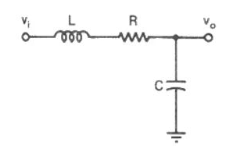
\includegraphics[scale=0.9]{171.png}
\caption{Dolní propust \cite{9}}
\end{figure}
\noindent Mezní frekvence a činitel jakosti tohoto obvodu byly spočítány jako 
\begin{align}
\omega _c &= \sqrt{\frac{1}{LC}}\\
Q &= \frac{L\sqrt{\frac{C}{L}}}{RC}.
\end{align}
Zapojení obvodu v Multisimu ilustruje Obrázek 15.
\begin{figure}[H]
\centering
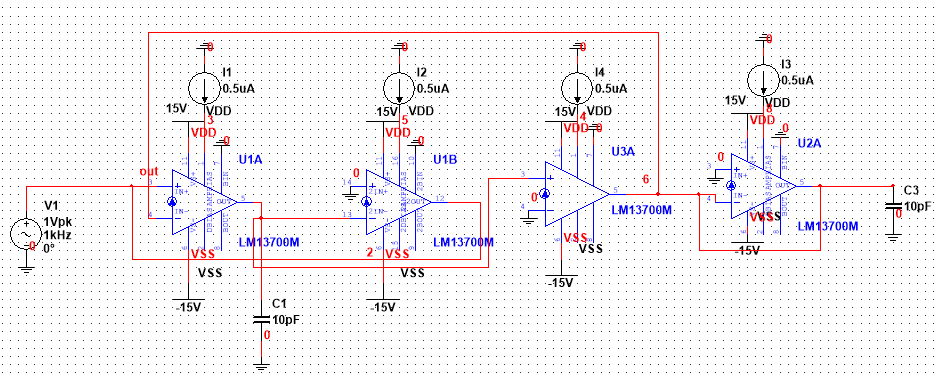
\includegraphics[scale=0.5]{1707.png}
\caption{Schéma zapojení dolní propusti 2. řádu}
\end{figure}
\begin{figure}[H]
\centering
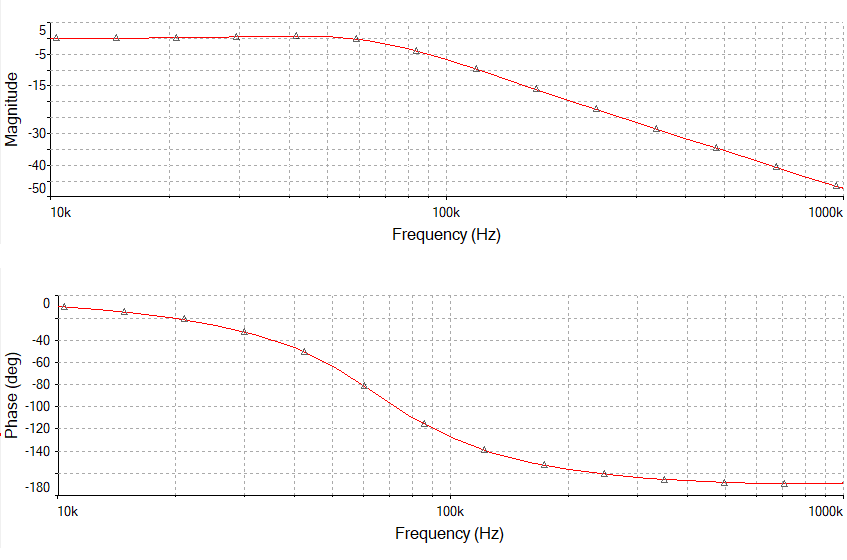
\includegraphics[scale=0.6]{17072.png}
\caption{Amplitudová a fázová charakteristika dolní propusti 2. řádu}
\end{figure}
\noindent Lze použít i zapojení z kapitoly 4 s uzemněným kapacitorem a odporem, avšak při této realizaci dochází v amplitudové charakteristice k překmitu. Proto bylo zvoleno řešení zmíněné výše.
\section{Dolní propust 4. řádu}
Kaskádní zapojení je realizováno násobením sériově zapojených bloků.
\begin{figure}[H]
\centering
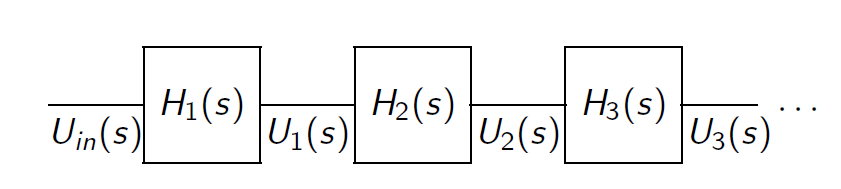
\includegraphics[scale=0.4]{schemata.png}
\caption{Kaskádní zapojení \cite{4}}
\end{figure}
Přenosové funkce jednotlivých bloků se násobí
\begin{align}
H_k(j\omega) = \frac{U_k (j\omega)}{U_{k-1}(j\omega)}.
\end{align}
Přenos posledního bloku je dán vztahem
\begin{align}
H_{1 \rightarrow k}(j\omega) = \frac{U_k (j\omega)}{U_{in}(j\omega)} = \prod _{n=1}^{k} H_n(j\omega).
\end{align}
Kaskádním zapojením dvou dolních propusti ze sekce 5 byl obdržen filtr 4. řádu s poklesem -80 dB/dek. 
\begin{figure}[H]
\centering
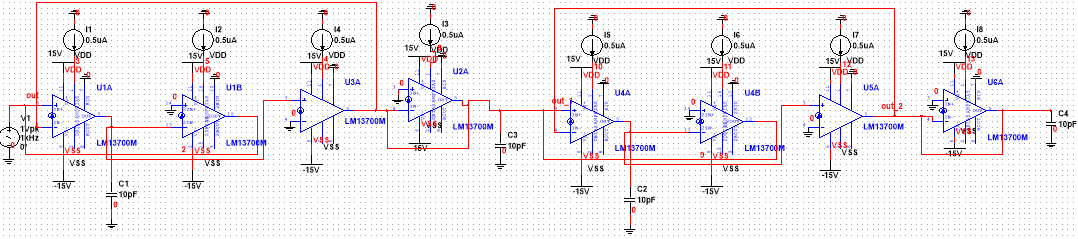
\includegraphics[scale=0.6]{lrcx2.png}
\caption{Schéma kaskádního zapojení dolní propusti 4. řádu}
\end{figure}
\begin{figure}[H]
\centering
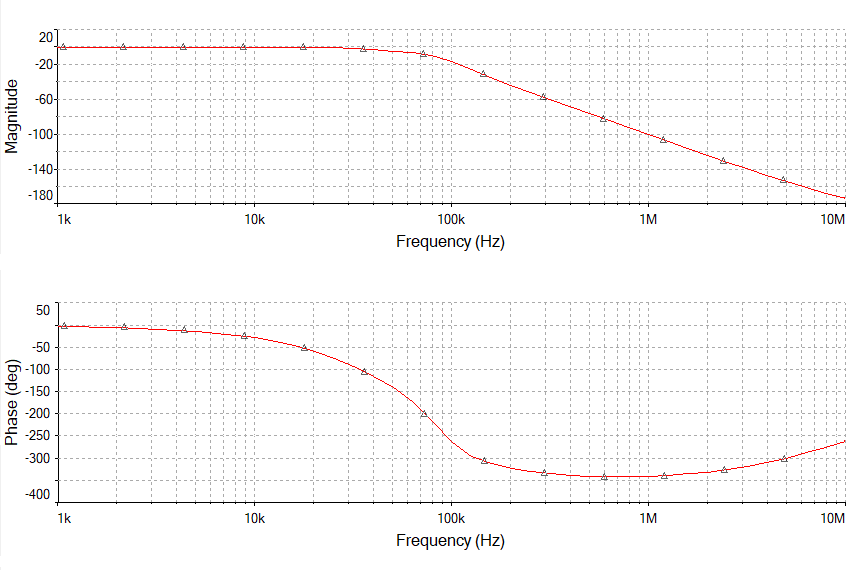
\includegraphics[scale=0.6]{lrcx2ampl.png}
\caption{Amplitudová a fázová charakteristika káskádního zapojení dolní propusti 4. řádu}
\end{figure}
\section{Pásmová propust 2. řádu}
Horní propust druhého řádu má přenos v nule nulový $H_{0} = 0$. Přenosová funkce je
\begin{align}
H(j\omega) = \frac{H_{\infty} (j\omega) ^2}{(j\omega)^2 + \frac{\omega _c}{Q}(j\omega) + \omega _c ^2}.
\end{align}
\noindent Pásmovou propust lze získat kaskádním zapojením dolní a horní propusti.
\begin{figure}[H]
\centering
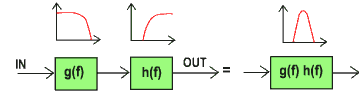
\includegraphics[scale=0.9]{fig9.png}
\caption{Násobení přenosů \cite{10}}
\end{figure}
\noindent Pásmová propust má přenos v nule i nekonečnu nulový $H_{0} = H_{\infty} = 0$. Přenosová funkce je
\begin{align}
H(j\omega) = \frac{H_{B} \frac{\omega _c}{Q} (j\omega) }{(j\omega)^2 + \frac{\omega _c}{Q}(j\omega) + \omega _c ^2}.
\end{align}
\noindent Nejprve byla zapojením dvou RC článků obdržena horní propust. Následně byla sériovým zapojením dolní a horní propusti 2. řádu obdržena pásmová propust 2. řádu.
\begin{figure}[H]
\centering
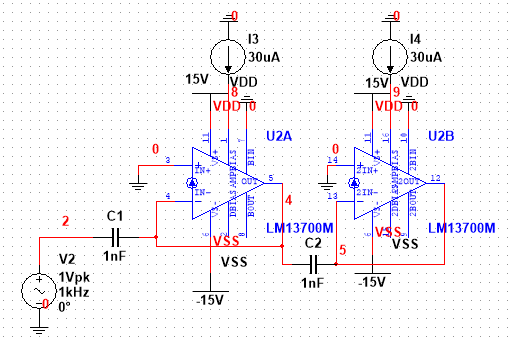
\includegraphics[scale=0.6]{1606.png}
\caption{Schéma zapojení horní propusti 2. řádu}
\end{figure}
\begin{figure}[H]
\centering
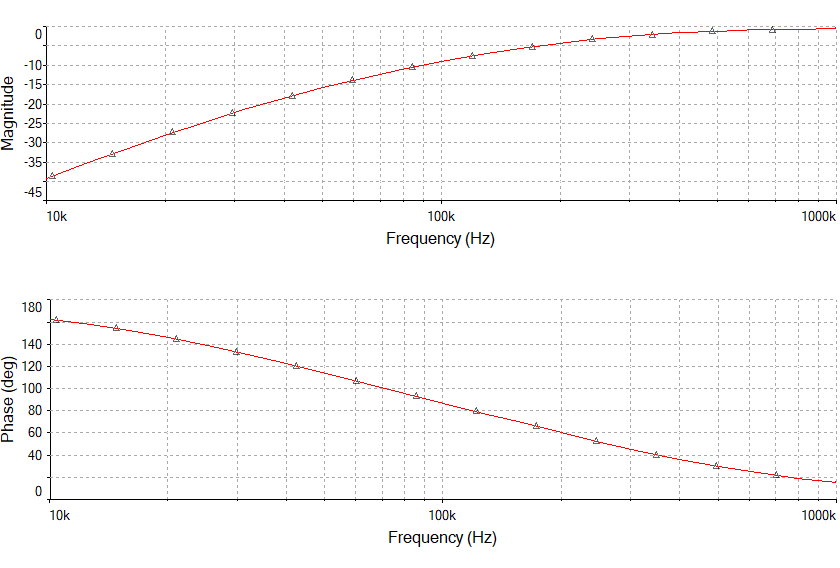
\includegraphics[scale=0.6]{16063.png}
\caption{Amplitudová a fázová charakteristika horní propusti 2. řádu}
\end{figure}
\begin{figure}[H]
\centering
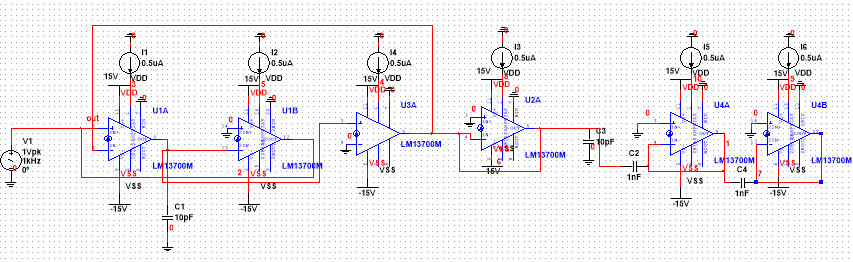
\includegraphics[scale=0.6]{lrcbandpass.png}
\caption{Schéma kaskádního zapojení pásmové propusti 2. řádu}
\end{figure}
\begin{figure}[H]
\centering
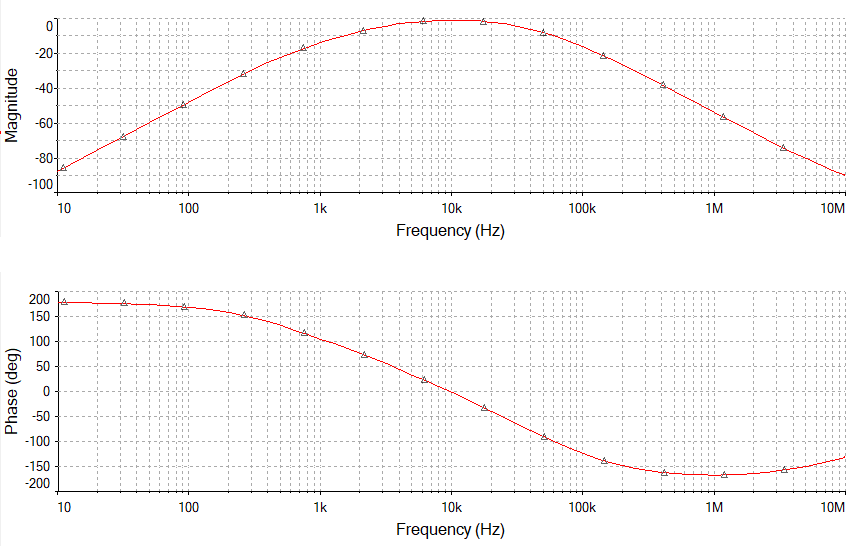
\includegraphics[scale=0.6]{lrcbandpassampl.png}
\caption{Amplitudová a fázová charakteristika káskádního zapojení pásmové propusti 2. řádu}
\end{figure}
\noindent Obvod je realizován zapojením odporu (Obrázek 10), kapacitoru a uzemněné indukčnosti(Obrázek 12).
\begin{figure}[H]
\centering
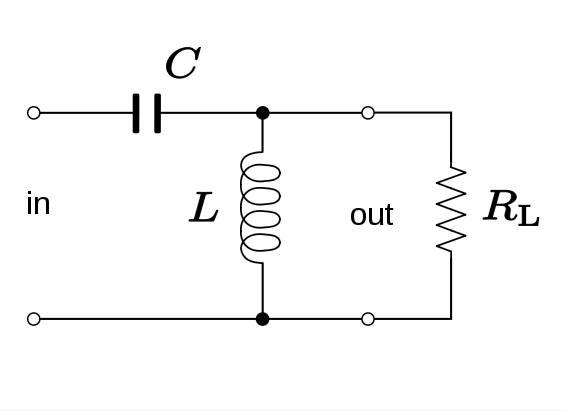
\includegraphics[scale=0.35]{high-pass.png}
\caption{Horní propust \cite{11}}
\end{figure}
\noindent Mezní frekvence a činitel jakosti tohoto obvodu byly spočítány jako 
\begin{align}
\omega _c &= \frac{1}{\sqrt{LC}}\\
Q &= \frac{1}{2 \zeta},
\end{align}
\noindent kde $\zeta$ je relativní útlum vyjádřený z přenosové funkce
\begin{align}
H(s) = \frac{s^2}{s^2 + 2 \zeta \omega _c s + \omega _c^2}.
\end{align}
\begin{figure}[H]
\centering
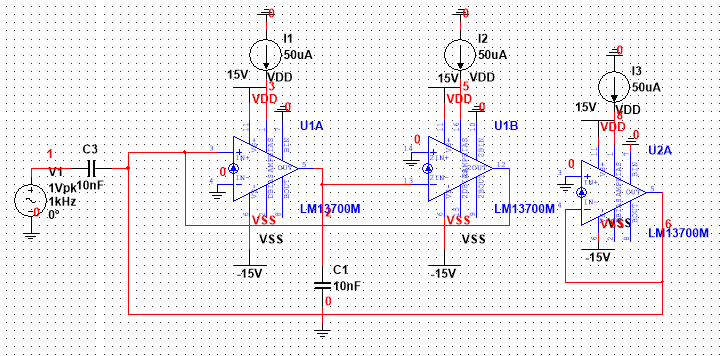
\includegraphics[scale=0.6]{hpsch.png}
\caption{Schéma zapojení horní propusti 2. řádu}
\end{figure}
\begin{figure}[H]
\centering
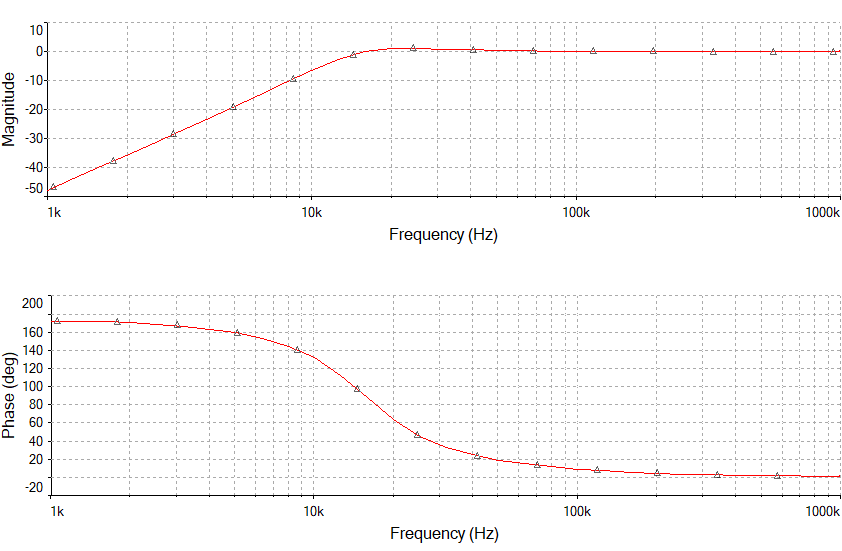
\includegraphics[scale=0.6]{hp.png}
\caption{Amplitudová a fázová charakteristika horní propusti 2. řádu}
\end{figure}
\begin{figure}[H]
\centering
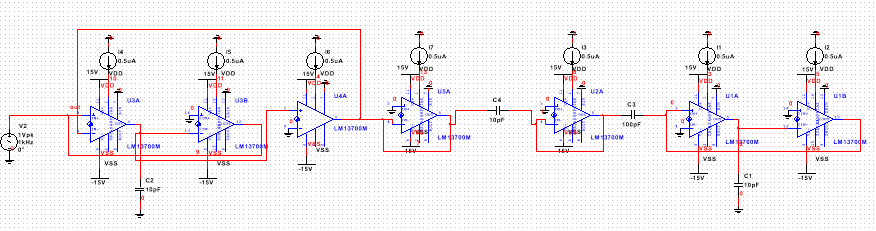
\includegraphics[scale=0.6]{bp2.png}
\caption{Schéma kaskádního zapojení pásmové propusti 2. řádu}
\end{figure}
\begin{figure}[H]
\centering
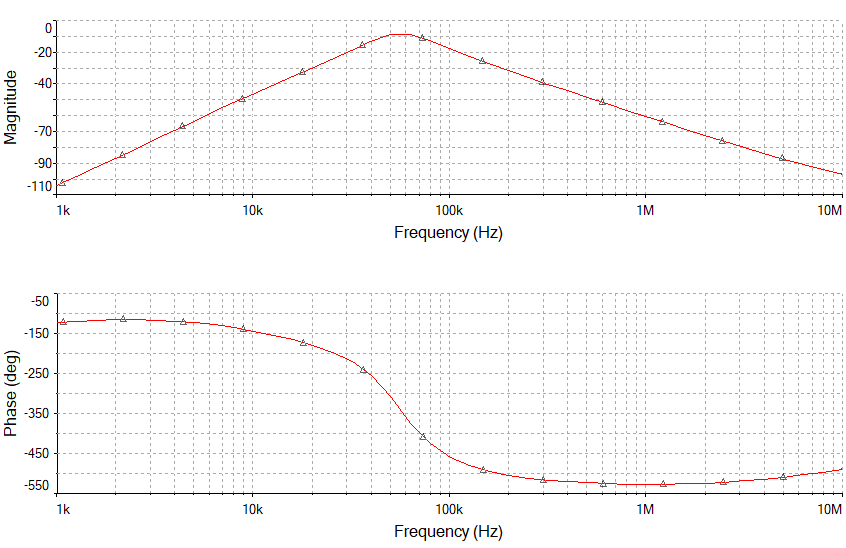
\includegraphics[scale=0.6]{bp22.png}
\caption{Amplitudová a fázová charakteristika káskádního zapojení pásmové propusti 2. řádu}
\end{figure}
\section{Pásmová propust 4. řádu}
\noindent Sériovým zapojením indukčnosti, odporu a uzemněného kapacitoru jako dolní propusti 4. řádu a následným zapojením dvou horních propustí 2. řádu byla obdržena pásmová propust 4.řádu. Byl obdržen filtr 4. řádu s poklesem -80 dB/dek. Průběh v okolí 0 dB není zcela hladký, protože hodnoty prvků v obvodu nebyly zvoleny přesně.
\begin{figure}[H]
\centering
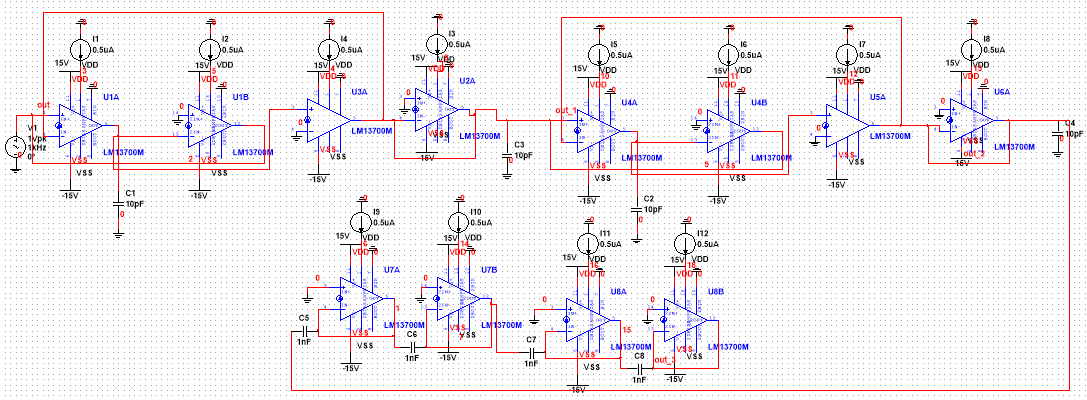
\includegraphics[scale=0.5]{lrcbandpass4.png}
\caption{Schéma kaskádního zapojení pásmové propusti 4. řádu}
\end{figure}
\begin{figure}[H]
\centering
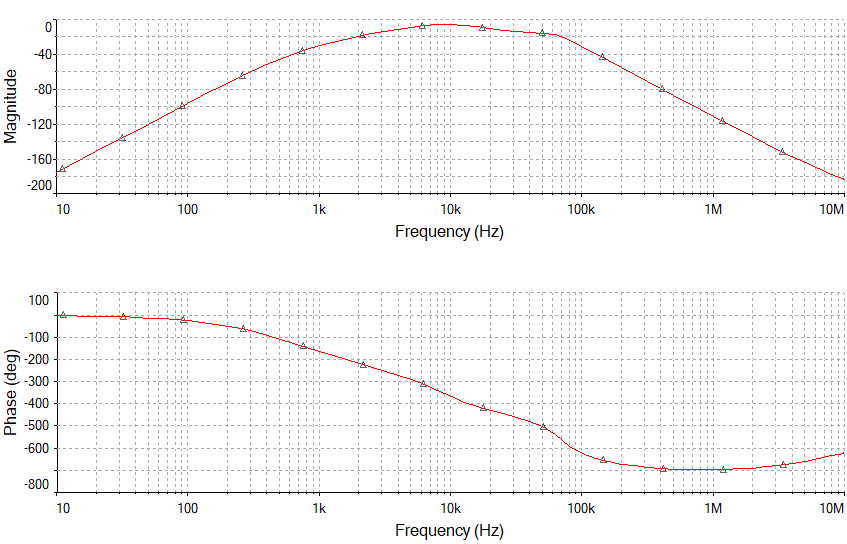
\includegraphics[scale=0.6]{lrcbandpass4ampl.png}
\caption{Amplitudová a fázová charakteristika káskádního zapojení pásmové propusti 4. řádu}
\end{figure}
\begin{figure}[H]
\centering
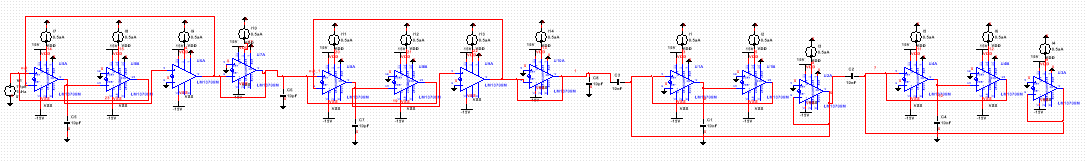
\includegraphics[scale=0.5]{bp4sch.png}
\caption{Schéma kaskádního zapojení pásmové propusti 4. řádu}
\end{figure}
\begin{figure}[H]
\centering
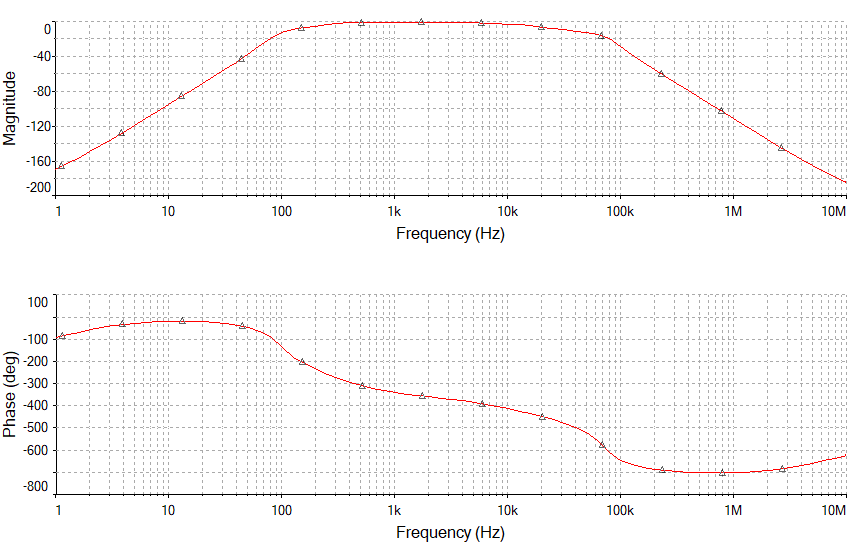
\includegraphics[scale=0.6]{bp42.png}
\caption{Amplitudová a fázová charakteristika káskádního zapojení pásmové propusti 4. řádu}
\end{figure}
\noindent Přeladěním na vyšší frekvenci byl obdržen následující průběh.
\begin{figure}[H]
\centering
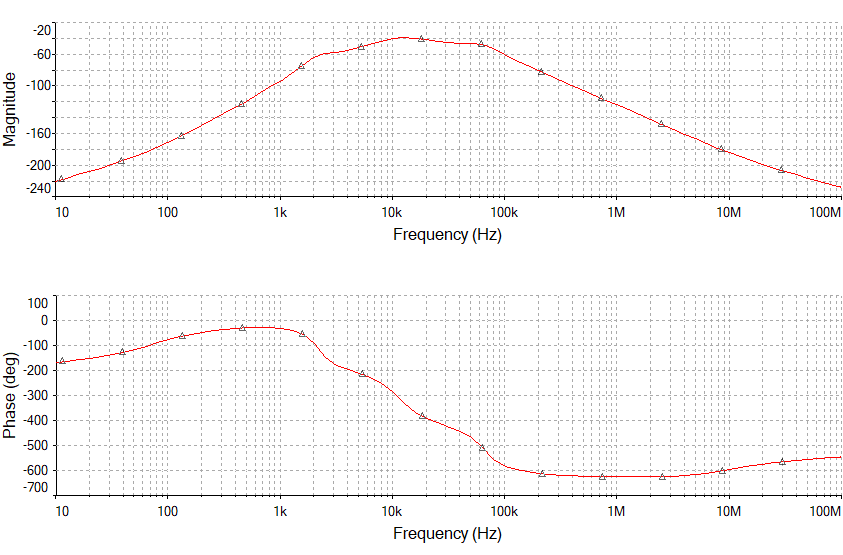
\includegraphics[scale=0.6]{bp4.png}
\caption{Amplitudová a fázová charakteristika káskádního zapojení pásmové propusti 4. řádu}
\end{figure}
\section{Příčkové LC filtry}
Pasivní dolní propust je realizována zapojením induktoru ke vstupnímu napětí a k této větvi je následně zapojen paralelně rezistor. Pasivní horní propust má ke vstupu připojený sériově rezistor a poté k této větvi paralelně induktor. \\
K realizaci filtrů vyšších řádů se užívají $\pi$ nebo T články s LC prvky. Při návrhu filtru musí být zohledněn vnitřní odpor zdroje $R_s$ a zatěžovací odpor $R_L$. LC filtry jsou tedy dvojitě zakončeny. Indukčnosti a kapacity prvků se určí z rovnic pro normované kapacity a indukčnosti. Normované hodnoty budou vypočteny pro mezní kmitočet $\omega _c = \frac{1}{\sqrt{LC}}$ a pro zatěžovací odpor $R_L$. Hodnoty prvků lze pro požadovanou aproximaci odečíst z tabulek. \\
\begin{figure}[H]
\centering
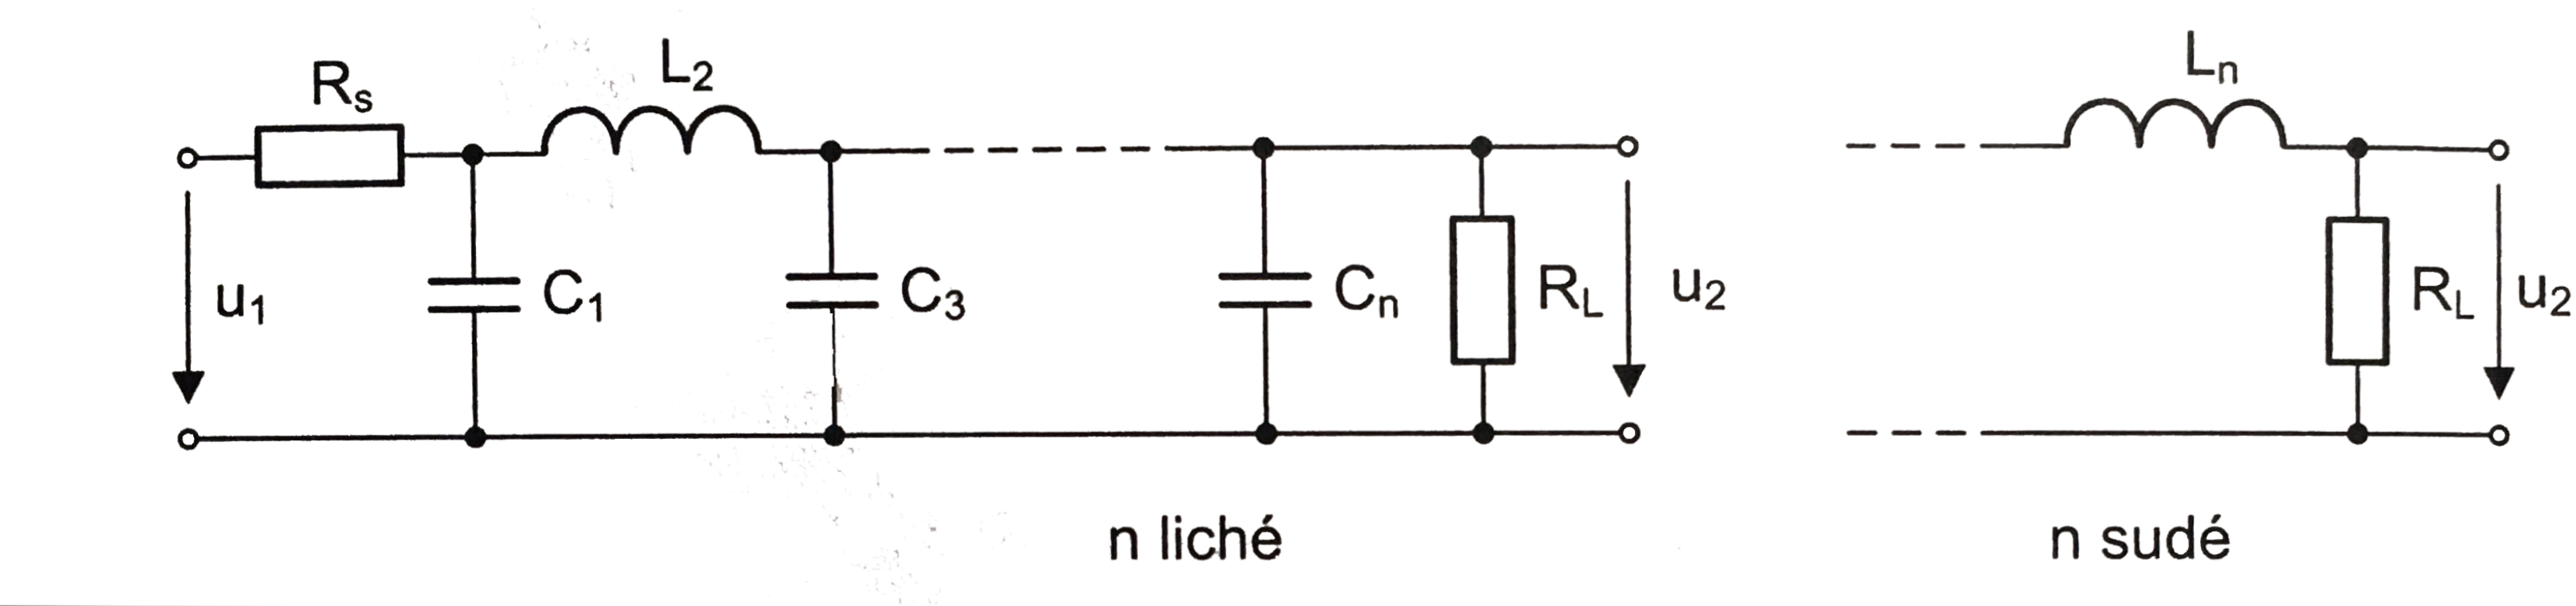
\includegraphics[scale=0.1]{piclanky.png}
\caption{Pasivní dolní propust n-tého řády s $\pi$ články \cite{12}}
\end{figure}
\begin{figure}[H]
\centering
\includegraphics[scale=0.08]{tclanky.png}
\caption{Pasivní dolní propust n-tého řády s T články \cite{12}}
\end{figure}
\begin{figure}[H]
\centering
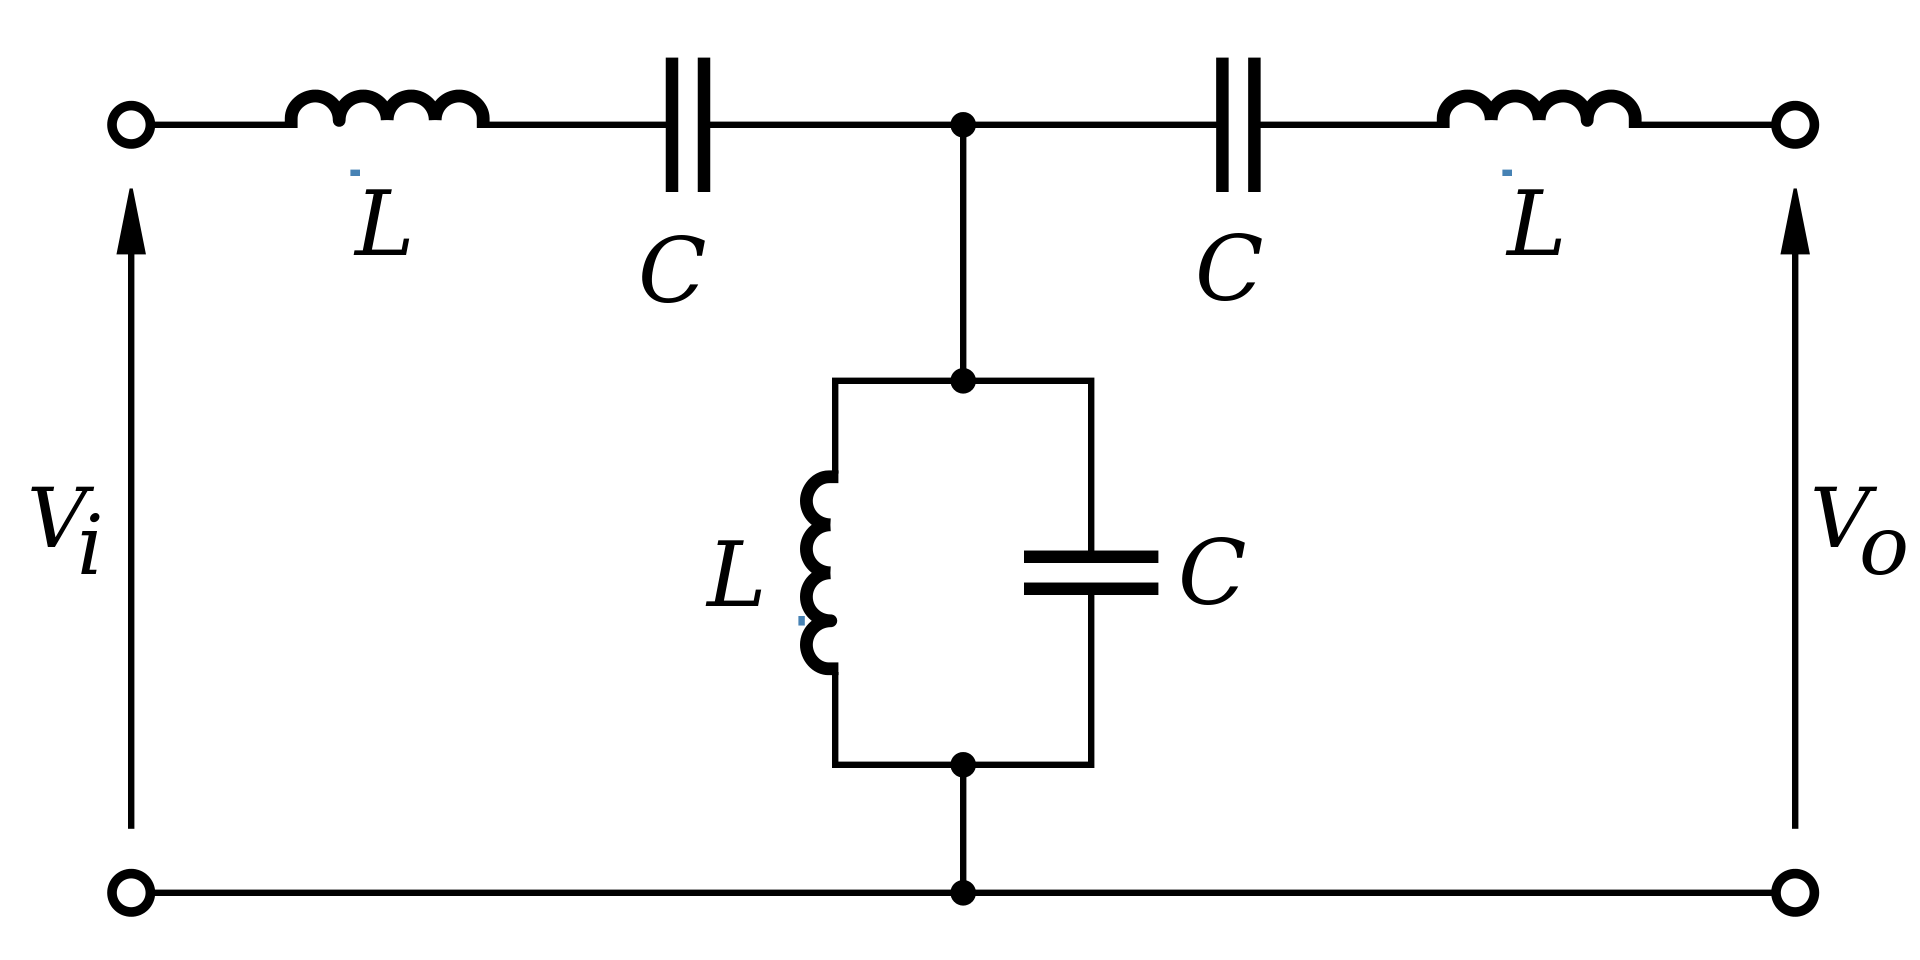
\includegraphics[scale=0.1]{Bandpass_Filter.png}
\caption{Zapojení pásmové propusti (T-článek) \cite{13}}
\end{figure}
\section{Návrh v Maple}
Pro návrh pásmové propusti 4. řádu s Cauerovou aproximací typu C byly zvoleny parametry tolerančního schématu 
\MapleOutput{fm := 80000 Hz}
\MapleOutput{delta\_{fp} := 130000 Hz}
\MapleOutput{delta\_{fs} := 300000 Hz}
\MapleOutput{ap := 20 dB}
\MapleOutput{as := 80  dB,}
\noindent kde $fm$ značí geometrický střed propustného pásma [Hz], $delta\_{fp}$ šířku propustného pásma [Hz],
$delta\_{fs} $ šířku nepropustného pásma [Hz], $ap$ maximální útlum v propustném pásmu [dB], $as$ minimální útlum v nepropustném pásmu [dB].
Funkcí $BP22NLP$ byla provedena transformace tolerančního schematu symetrické pásmové propusti (PP) na toleranční schema normované dolní propusti (NDP). Byly spočteny spodní a horní hranice nepropustného pásma $f\_s,fs$ a spodní a horní hranice propustného pásma $f\_p,fp$. 
\begin{align}
f\_s &= \frac{\sqrt{delta\_{fs}^2+4f\_m ^2}-delta\_{fs}}{2}\\
f\_p &= \frac{\sqrt{delta\_{fp}^2+4f\_m ^2}-delta\_{fp}}{2}\\
fp &= \frac{\sqrt{delta\_{fp}^2+4f\_m ^2}+delta\_{fp}}{2}\\
fs &= \frac{\sqrt{delta\_{fs}^2+4f\_m ^2}+delta\_{fs}}{2}
\end{align}
\MapleOutput{x:=BP22NLP(80e3,130e3,300e3,20,80)}
\MapleOutput{f\_s = 20000 Hz}
\MapleOutput{f\_p = 38077 Hz}
\MapleOutput{fp = 168077 Hz}
\MapleOutput{fs = 320000 Hz}
\noindent Byl obdržen kmitočet hranice nepropustného pásma normované dolní propusti (NDP) $Os$ [1/s].
\MapleOutput{Os = 2.30769 1/s}.
\begin{figure}[H]
\centering
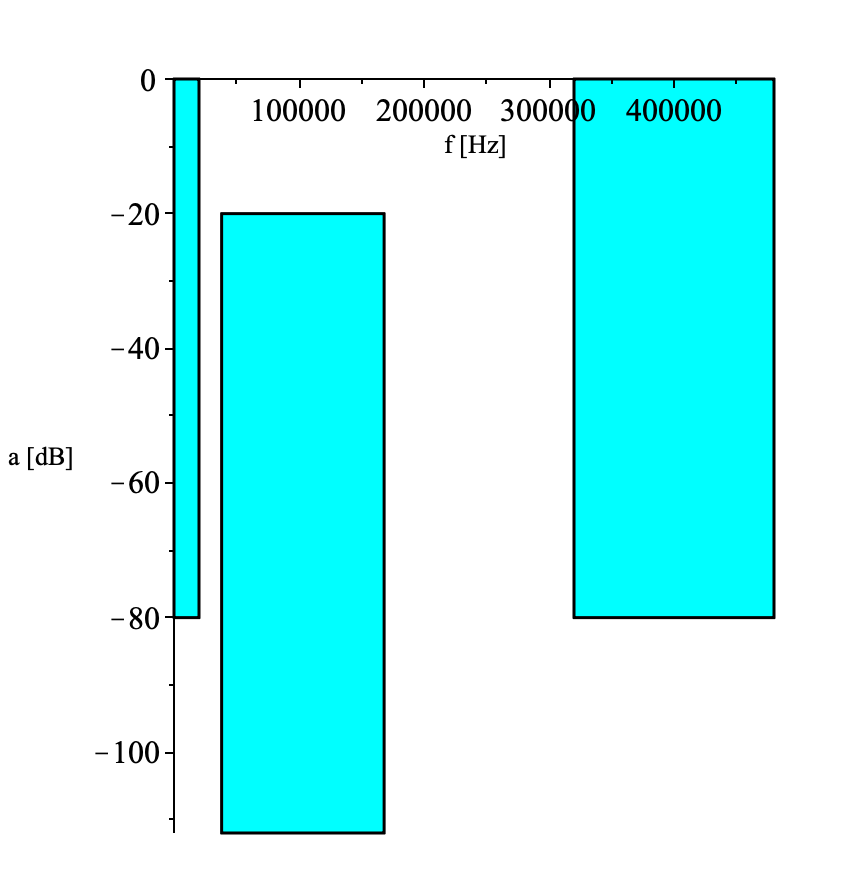
\includegraphics[scale=0.5]{tolsch.png}
\caption{Toleranční schéma navrhované pásmové propusti}
\end{figure}
\noindent Stupeň Cauerovy aproximace normované dolní propusti byl určen jako $order = 4$.
\MapleOutput{Nc:=CauerNLPOrder(Os)}
\MapleOutput{Nc := 4, 2.30769, 20}
\noindent Dále byla funkcí $Cauer\_asnew$ určena nová hodnota útlumu v nepropustném pásmu NDP $asnew$.
\MapleOutput{asnew := Cauer\_asnew(Nc)}
\MapleOutput{asnew := 83.3624}
\begin{align}
asnew&= 10log10(1 + ( \frac{\epsilon}{kl\_new})^2)\\
\epsilon &= \sqrt{10^{0.1ap} - 1)}\\
k &= \frac{1}{Os}\\
kl\_new &= k^{order}(\prod_{i=1}^{n}JacobiCD(\frac{(2i - 1 + m)EllipticK(k)}{order},k))^4,
\end{align}
\noindent kde $m$ je celočíselný zbytek po dělení řádu 2 a $n$ celočíselný výsledek dělení. Jakobiho eliptických funkcí je 12 a vycházejí ze škálování na jednotkové elipse (cos $\phi$, sin $\phi$ se neváží k jednotkovému kruhu, ale k elipse). JacobiCD funkce je definována jako podíl cosinu Jakobiho funkce s dvěma parametry (JacobiAM(z,k)) a derivace této funkce podle prvního parametru z.
\begin{align}
EllipticK(k) = \int _0 ^1(\frac{1}{\sqrt{(-\_ \alpha _1^2+1)}\sqrt{(-k^2 \_ \alpha _1^2+1})})d \_ \alpha _1
\end{align}
Následně byl spočten koeficient nejvyšší mocniny polynomu ve jmenovateli přenosové funkce $Gc$, póly a nuly přenosové funkce $poles, zeros$ pomocí funkce $CauerCPolesZeros$. Počet pólů je dán řádem filtru $order$ a počet nul pro aproximaci typu C je roven $order - 2$. Dále byla spočtena Caurerova aproximace typu C - provozní činitel přenosu $G$ jako racionální lomená funkce $G(j\omega) = \frac{1}{H(j\omega)}$, charakteristická funkce $chf$ jako $\Phi(j\omega)$ s nulami a póly na imaginární ose a nuly přenosu. Charakteristická funcke má shodný jmenovatel s $G(j\omega)$.
\MapleOutput{Gc,poles,zeros:=CauerCPolesZeros(Nc)}
\MapleOutput{G,chf,zer:=CauerC(Nc,p)}
\MapleOutput{Gc, poles, zeros := 459.404,}
\MapleOutput{[-0.106147+0.103691 I,-0.106147-0.103691 I,-0.0119965+0.915370 I,-0.0119965-0.915370 I],}
\MapleOutput{ [2.91159I -2.91159 I]}
\MapleOutput{G,chf,zer := \frac{459.404p^4+108.551p^3+397.458p^2+81.9762p+8.47734}{p^2+8.47736}, \frac{(459.404p^2+384.647)p^2}{p^2+8.47736}, [2.91159I -2.91159 I]}
\begin{figure}[H]
\centering
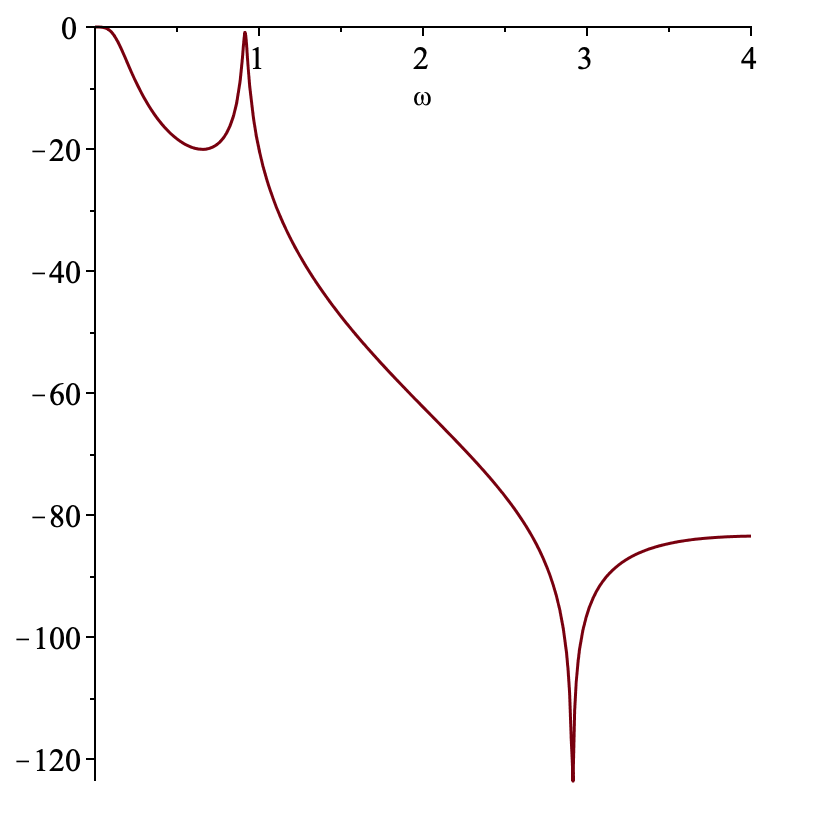
\includegraphics[scale=0.5]{sch.png}
\caption{Modulová frekvenční charakteristika NDP}
\end{figure}
\noindent Charakteristika byla vykreslena z přenosu funkcí $MagnitudeHdB$, která vypočte modul přenosu podle předpisu |H(j$\omega)$|.
\section{Výpočet prvků LC filtru}
\noindent Funkcí DroppNLP byly vypočteny prvky LC příčkového filtru typu normovaná dolní propust (NDP). Zakončení bylo zvoleno standardní (common), odpory o hodnotě 1 $\Omega$, směr zpracování od posledního prvku (rear), s T strukturou (začíná zepředu podélným induktorem). Standardní (common) zakončení je oboustranné ($R_1 != 0, R_1 != \infty$). Výstupem funkce je LC struktura s orientací prvků ve větvi podélně (direct) nebo příčně (shunt).
\MapleOutput{elems\_NLP:=DroppNLP('common',1,rear,T,G,chf,zer)}
\MapleOutput{             
Rem\_matrix = \begin{pmatrix} 1.00624  &  0 \\
0.  &  1.00150
\end{pmatrix}}
\MapleOutput{type = LC\_NLP\_common}
\MapleOutput{R1 = 1}
\MapleOutput{R2 = 1.004}
\MapleOutput{block (1), [orientation = direct, elements = {L1 = 27.298}, Z = p L1]}
\MapleOutput{block (2), [orientation = shunt, elements = {C1 = 1.6705}, Z = \frac{1}{pC1}]}
\MapleOutput{block (3), [orientation = direct, elements = {C1 = 0.14180, L1 = 0.83190}, Z = \frac{1}{\frac{1}{pL1} + pC1}]}
\MapleOutput{block (4), [orientation = shunt, elements = {C1 = 8.3068}, Z = \frac{1}{pC1}]}
\noindent Přenosová funkce pasivních a aktivních struktur filtru byla spočtena funkcí MakeH. Byl spočten  napěťový i výkonový přenos.
\MapleOutput{H\_NLPV := MakeH(elems\_NLP, V)}
\MapleOutput{H\_NLP := MakeH(elems\_NLP, P)}
\MapleOutput{H\_NLPV := \frac{p^2  + 8.47735}{2943.77 p^4  + 455.340 p^3  + 2381.21^2  + 322.099 p + 16.9209}   }
\MapleOutput{H\_NLP := \frac{0.999999 p^2  + 8.4773}{1474.83 p^4  + 228.125 p^3  + 1192.99 p^2  + 161.371 p + 8.47736}}
\begin{figure}[H]
\centering
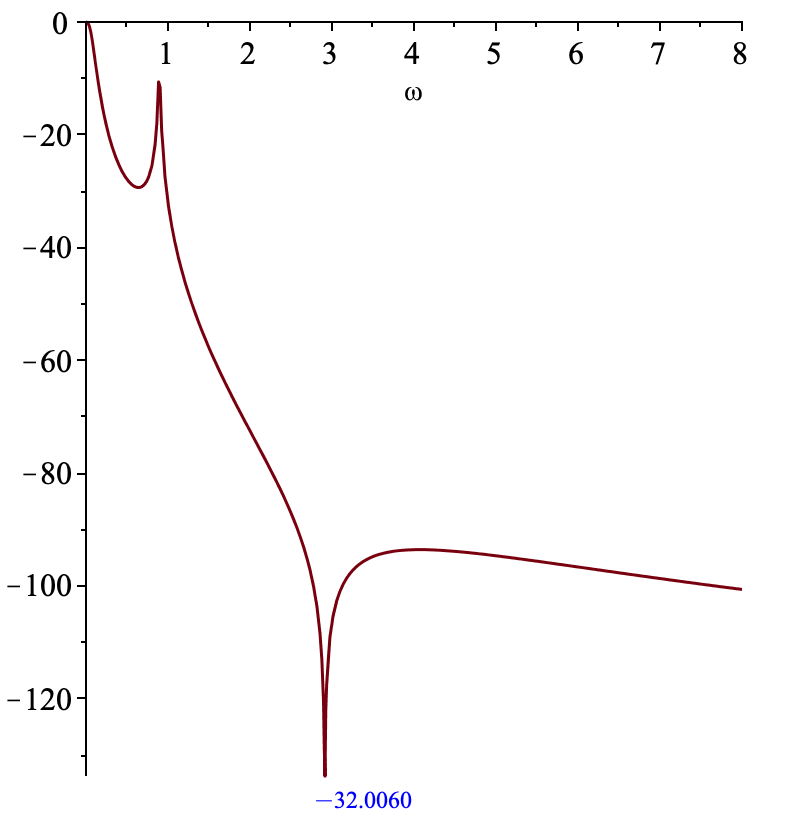
\includegraphics[scale=0.5]{sch2.png}
\caption{Modulová frekvenční charakteristika NDP - LC příčkový filtr}
\end{figure}
\noindent Hodnota přenosové funkce v 1 byla vyhodnocena jako $-32.006$.\\
Byla provedena transformace hodnot prvků normované dolní propusti (NDP) na pásmovou propust (PP). Zakončovací rezistor byl zvolen 1 $\Omega$, další dva parametry funkce značí spodní a horní hranici propustného pásma.
\MapleOutput{elems\_BP := ElemsBP(elems\_NLP, 1, 38077.640640, 168077.640640)}
\MapleOutput{type = LC\_BP\_common}
\MapleOutput{R1 = 1}
\MapleOutput{R2 = 1.004}
\MapleOutput{block (1), [Z = p L1 + \frac{1}{pC1}, orientation = direct, elements = { C1 = 1.1843*10^{-7}  , L1 = 3.3420*10^{-5}}]}
\MapleOutput{block (2), [Z = \frac{1}{\frac{1}{pL1}+pC1}, orientation = shunt, elements = {C1 = 2.0451 *10^{-6}, L1 = 1.9353*10^{-6}}]}
\MapleOutput{block (3), [Z = \frac{1}{pC1 + \frac{1}{pL1}+\frac{1}{pL2 + \frac{1}{pC2}}} orientation = direct, elements = { C1 = 1.7360*10^{-7} ,}}
\MapleOutput{C2 = 3.8861*10^{-6}, L1 = 2.2799*10^{-5}, L2 = 1.0185*10^{-6}]}
\MapleOutput{block (4), [Z = \frac{1}{\frac{1}{pL1}+pC1}, orientation = shunt, elements = { C1 = 1.0170 *10^{-5}, L1 = 3.8918*10^{-7}}]}
\noindent Byly nastaveny jakosti cívek v LC příčkové struktuře na konečnou hodnotu. Funkce $MakeRealL$ zařadí do výsledné LC příčkové struktury sériově rezistory k induktorům podle zadaného činitele jakosti $Q$ a zadaného kmitočtu (ten odpovídá u pásmové propusti geometrickému středu propustného pásma - nebo je možno zadat obě hranice propustného pásma). Výpočet sériového odporu je proveden podle předpisu $R_s = \frac{L1 . 2 \pi f}{Q}$.
\MapleOutput{Q:=50:}
\MapleOutput{elems\_BPQ:=MakeRealL(elems\_BP,Q,38077.640640, 168077.640640):}
\MapleOutput{type = LC\_BP\_common\_Q}
\MapleOutput{R1 = 1}
\MapleOutput{R2 = 1.004}
\MapleOutput{block (1), [Z = p L1 + Rs1 + \frac{1}{pC1}, orientation = direct, elements = { C1 = 1.1843*10^{-7}  , L1 = 3.3420*10^{-5}, }}
\MapleOutput{Rs1 = 0.33598]}
\MapleOutput{block (2), [Z = \frac{1}{\frac{1}{pL1 + Rs1}+pC1}, orientation = shunt, elements = {C1 = 2.0451 *10^{-6}, L1 = 1.9353*10^{-6},}}
\MapleOutput{Rs1 = 0.019455]}
\MapleOutput{block (3), [Z = \frac{1}{pC1 + \frac{1}{pL1 + Rs1}+\frac{1}{pL2 + Rs2 + \frac{1}{pC2}}} orientation = direct, elements = { C1 = 1.7360*10^{-7} ,}}
\MapleOutput{C2 = 3.8861*10^{-6}, L1 = 2.2799*10^{-5}, L2 = 1.0185*10^{-6}, Rs1 = 0.2292, Rs2 = 0.010239]}
\MapleOutput{block (4), [Z = \frac{1}{\frac{1}{pL1 + Rs1}+pC1}, orientation = shunt, elements = { C1 = 1.0170 *10^{-5}, L1 = 3.8918*10^{-7}, }}
\MapleOutput{Rs1 = 0.0039125]}
\noindent Byl spočten přenos pro LC strukturu bez a s přidanými sériovými rezistory. Pro oba přenosy byla vykreslena modulová frekvenční charakteristika.
\MapleOutput{H\_BP:=MakeH(elems\_BP);}
\MapleOutput{H\_BPQ:=MakeH(elems\_BPQ);}
\begingroup
    \fontsize{5pt}{12pt}
\MapleOutput{H\_BP := \frac{ p^6  + 6.1612* 10^{12}   p^4  + 6.38385 *10^{22}  p^2}{2.21053
  10^{-9}  p^8  + 0.000279286 p^7  + 3427.09 p^6  + 3.43505 *10^{8}   p^5 + 1.45520* 10^{15} p^4  + 8.67913 10^{19} p^3  + 2.18778*10^{26} p^2 + 4.50478 *10^{30} p + 9.00862 *10^{36} }}
\MapleOutput{H\_BPQ := \frac{p^7  + 40212.3 p^6 + 6.16193*10^{12}  p^5 + 1.85826*10^{17}p^4+6.57069*10^{22}p^3+1.28981*10^{27}p^2 + 6.45184 10^{30} p}{2.21053*10^{-9}p^9 +0.000390400 p^8+3442.71 p^7+4.81598*10^8 p^6+1.47026*10^{15} p^5+1.30876*10^{20} p^4+2.21624*10^{26} p^3+8.92708*10^{30} p^2+9.11067*10^{36} p +9.09122*10^{40} }}
\endgroup
\begin{figure}[H]
\centering
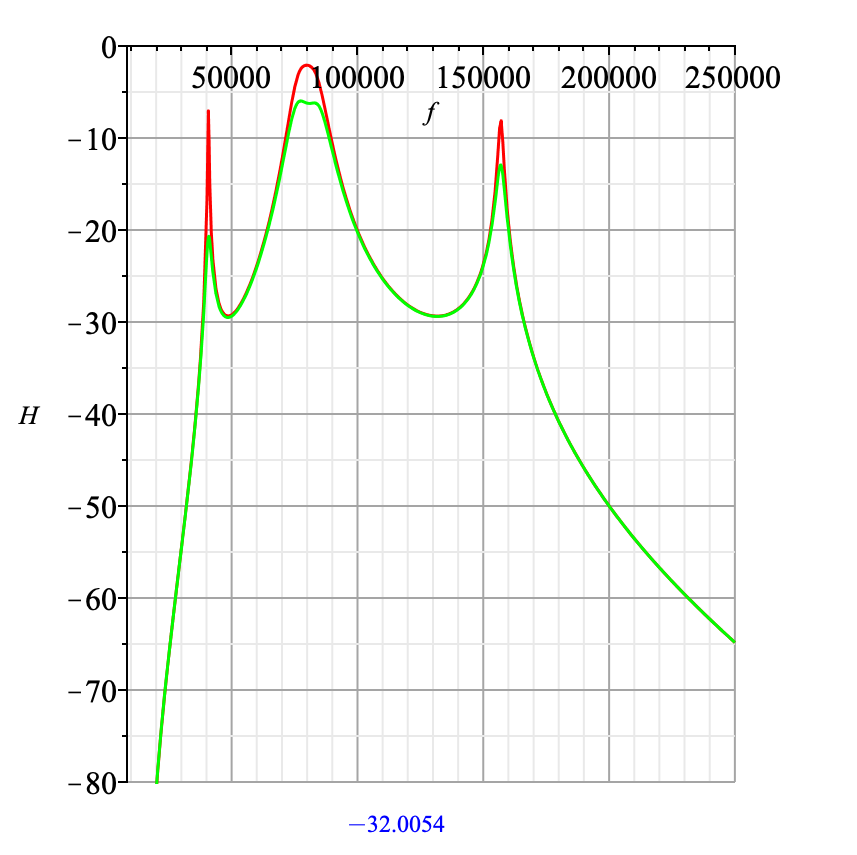
\includegraphics[scale=0.6]{modul1.png}
\caption{Modulová frekvenční charakteristika LC struktury (červená) a LC struktury s končnou hodntou jakostí cívek (zelená)}
\end{figure}
\noindent Vyčíslením v $168077*2 \pi$ Hz byl obdržen útlum 32 dB.\\
\\
Odnormované prvky byly vyčísleny následovně:
\MapleOutput{ele\_BP:={L1=subs(eval(elems\_BPQ[1][elements]),L1), C1=subs(eval(elems\_BPQ[1][elements]),C1),}}
\MapleOutput{C2=subs(eval(elems\_BPQ[2][elements]),C1), L2=subs(eval(elems\_BPQ[2][elements]),L1),}
\MapleOutput{L3=subs(eval(elems\_BPQ[3][elements]),L2), L4=subs(eval(elems\_BPQ[3][elements]),L1),} \MapleOutput{C3=subs(eval(elems\_BPQ[3][elements]),C2), C4=subs(eval(elems\_BPQ[3][elements]),C1),}
\MapleOutput{C5=subs(eval(elems\_BPQ[4][elements]),C1),L5=subs(eval(elems\_BPQ[4][elements]),L1),}
\MapleOutput{R0=eval(elems\_BPQ)[R1], Rz=eval(elems\_BPQ)[R2];}
\MapleOutput{ele\_BP := { C1 = 1.18426*10^{-7}  , C2 = 2.04513*10^{-6},  C3 = 3.88609*10^{-6} , C4 = 1.73599 *10^{-7},}}
\MapleOutput{ C5 = 10.1698*10^{-6}, L1 = 0.0000334204, L2 = 0.00000193526, L3 = 0.00000101846, L4 = 0.0000227988, }
\MapleOutput{L5 = 3.89179 *10^{-7}, R0 = 1, Rz = 1.004}
\noindent Kapacita kondenzátoru použitého při zapojení indukčnosti s OTA je rovna $C_L = L g_m ^2$. Byla uvažována minimální transkonduktance z datasheetu LM13700. Byly získány kapacity
\MapleOutput{C_{L1} = 3.080024064*10^{-9}, C_{L2} = 1.783535616*10^{-10}, C_{L3} = 9.38612736*10^{-11}, C_{L4} = 2.101137408 *10^{-9},}
\MapleOutput{C_{L5} = 3.586673664*10^{-11}},
\noindent tedy $C_{L1} = 3.08002$ nF, $C_{L2} = 178.35356$ pF, $C_{L3} = 93.86127$ pF, $C_{L4} = 2.10114$ nF, $C_{L5} = 35.86674$ pF.
\noindent Převrácenou hodnotou transkonduktance byly vypočteny frekvenčně a impedančně odnormované odpory
\begin{align}
R_N = R_0 = R_z = \frac{1}{g_m} = 104.16667 \Omega.
\end{align}
\noindent Kapacity vyšly odnormovány již se Syntfilu $C1 = 118.426$ nF, $C2 = 2.04513$ uF, $C3 = 3.88609$ uF, $C4 = 173.599$ nF, $C5 = 10.1698$ uF.
\section{Simulace s výsledky ze Syntfilu}
\noindent Vypočtené prvky byly dosazeny do schématu v Multisimu. Bylo použito zapojení se vstupním odporem $R_0$ řazeným paralelně ke zdroji (vhodnější pro funkční simulaci - Schaumann (2001) str. 656/758). Napětí na zdroji poté bude $\frac{V_0}{R_0}$.
\begin{figure}[H]
\centering
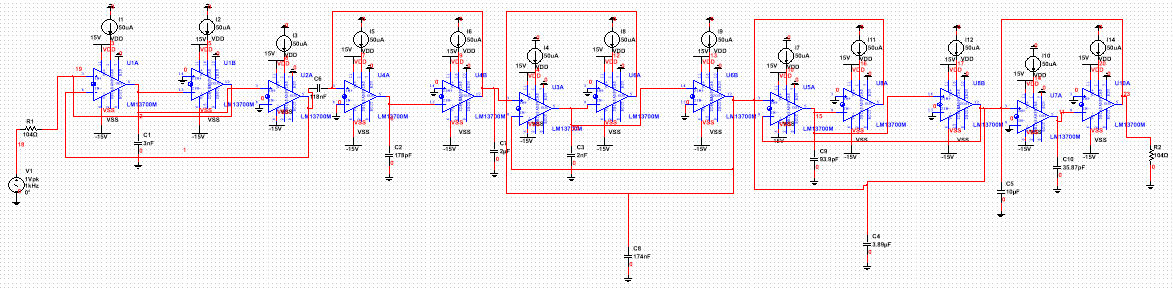
\includegraphics[scale=0.55]{maple.png}
\caption{Zapojení pásmové propusti (Syntfil)}
\end{figure}
\begin{figure}[H]
\centering
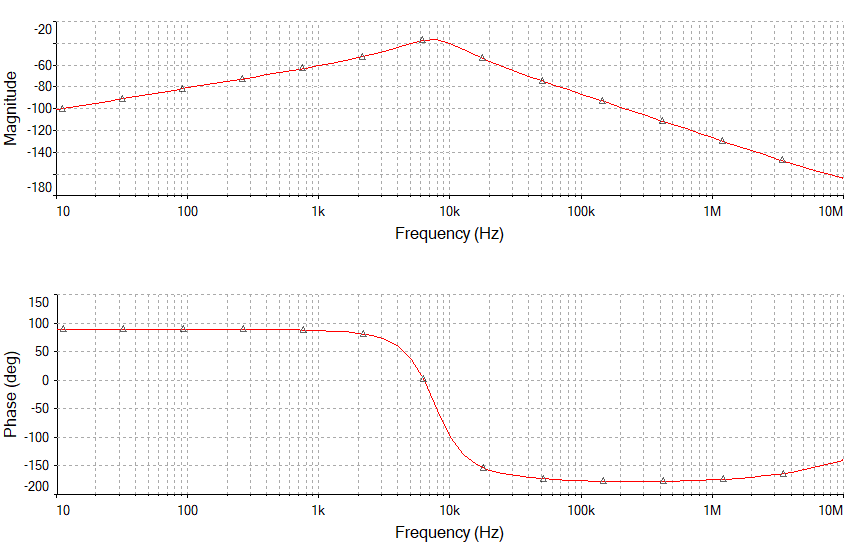
\includegraphics[scale=0.6]{maple2.png}
\caption{Amplitudová a fázová charakteristika pásmové propusti (Syntfil)}
\end{figure}
\begin{figure}[H]
\centering
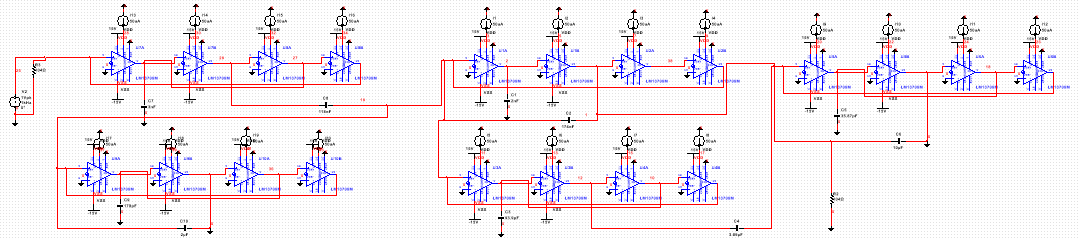
\includegraphics[scale=0.55]{maple4.png}
\caption{Zapojení pásmové propusti (Syntfil)}
\end{figure}
\begin{figure}[H]
\centering
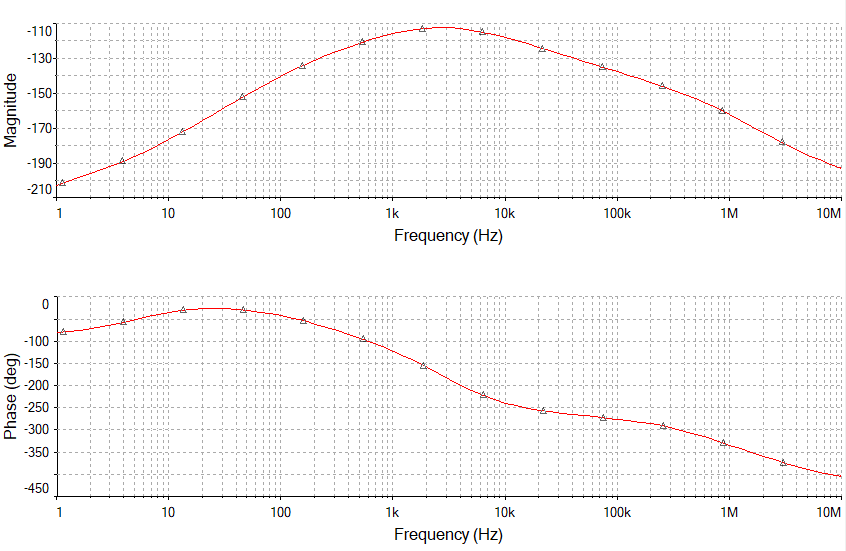
\includegraphics[scale=0.6]{maple42.png}
\caption{Amplitudová a fázová charakteristika pásmové propusti (Syntfil)}
\end{figure}
\section{Návrh funkční simulací}
\begin{figure}[H]
\centering
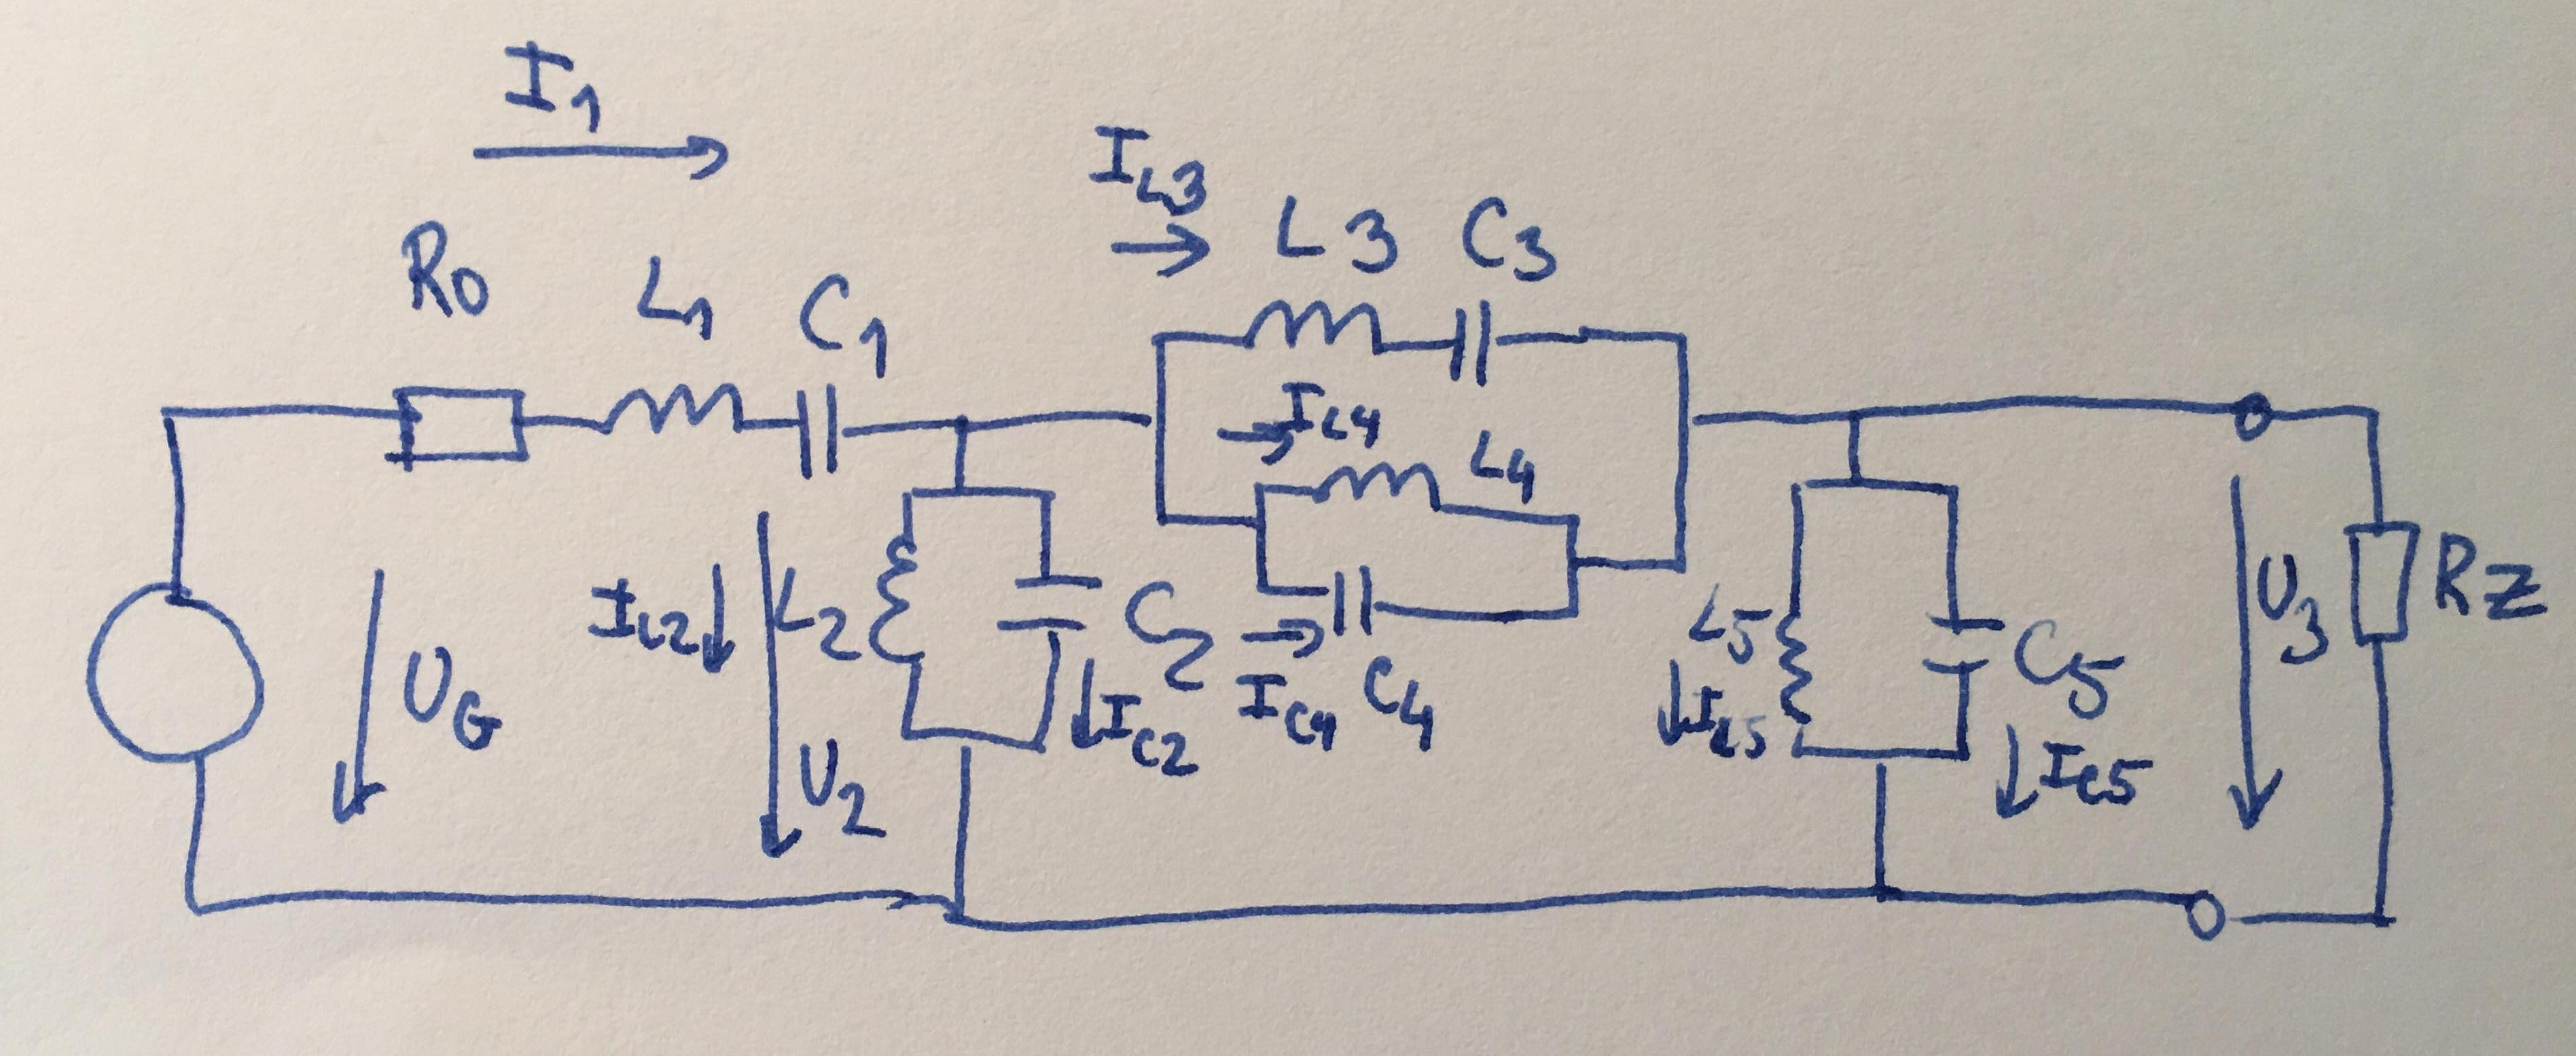
\includegraphics[scale=0.08]{LCstruktura.png}
\caption{Schéma LC příčkové struktury}
\end{figure}
\noindent Analýzou LC struktury z Maplu byly obdrženy obvodové rovnice, kde R je volitelný (fiktivní) rezistor:
\begin{align}
I_1 &= \frac{1}{R_1 + pL_1 + \frac{1}{pC_1}}(U_G - U_2)\\
v_1 & = \frac{R}{R_1 + pL_1 + \frac{1}{pC_1}}(U_G - U_2)\\
U_2 &= \frac{pL_1}{\frac{1}{pL_1} + pC_1}(I_1 - I_{L3} - I_{L4} - pC_4 v_{L4})\\
U_2 &= \frac{pL_1}{\frac{R}{pL_1} + RpC_1}(v_1 - v_{L3} - v_{L4} - RpC_4 U_{L4})\\
I_{L3} &= \frac{1}{pL_3 + \frac{1}{pC_3}}(U_2 - U_3)\\
v_{L3} &= \frac{R}{pL_3 + \frac{1}{pC_3}}(U_2 - U_3)\\
v_{L4} &= \frac{1}{\frac{1}{pL_4}+pC_4}(I_1 - I_{L2} - pC_2U_2 - I_{L3} - pC_4 (U_2 - U_3))\\
v_{L4} &= \frac{1}{\frac{R}{pL_4}+RpC_4}(v_1 - v_{L2} - RpC_2U_2 - v_{L3} - RpC_4 (U_2 - U_3))\\
U_3 &= \frac{1}{\frac{1}{R_z}+pC_5 + \frac{1}{pL_5}}(I_1 - I_{L2} - pC_2U_2 - I_{L3} - I_{L4} - pC_4 v_{L4})\\
U_3 &= \frac{1}{\frac{R}{R_z}+RpC_5 + \frac{R}{pL_5}}(v_1 - U_2 - RpC_2 U_2 - v_{L3} - v_{L4} - RpC_4 v_{L4}).
\end{align}
\noindent To odpovídá realizační struktuře s pěti gyrátory o přenosech $H_1...H_5$
\begin{align}
H_1 & = \frac{R}{R_1 + pL_1 + \frac{1}{pC_1}}\\
H_2 &= \frac{pL_1}{\frac{R}{pL_1} + RpC_1}\\
H_3 &= \frac{R}{pL_3 + \frac{1}{pC_3}}\\
H_4 &= \frac{1}{\frac{R}{pL_4}+RpC_4}\\
H_5 &= \frac{1}{\frac{R}{R_z}+RpC_5 + \frac{R}{pL_5}}.
\end{align}
\noindent Dosazením za přenos ztrátového integrátoru (byly uvažovány stejné gm)
\begin{align}
H & = \frac{gm}{sc + gm}
\end{align}
a porovnáním s předchozími přenosy $H_1...H_5$ byly obdrženy následující hodnoty
\MapleOutput{CI := [{CI1 = -\frac{gm*(H1-1)}{(H1*s)}, CI2 =\frac{ gm*(C1*L1*R1*p^2-L1^2*p^2+R1)}{(L1^2*p^2*s)}, CI3 = \frac{gm*(C3*L3*p^2-C3*R1*p+1)}{(C3*R1*p*s)}, }}
\MapleOutput{CI4 = \frac{gm*(C4*L4*R1*p^2-L4*p+R1)}{(L4*p*s)}, CI5 = \frac{gm*(C5*L5*R1*Rz*p^2+L5*R1*p-L5*Rz*p+R1*Rz)}{(L5*Rz*p*s)}]}
\noindent Zohledněním paralelního zapojení kondenzátoru C2, C4 a C5 k indukčnosti bylo dosazeno za původní hodnoty dosazeno $Cg=C*gm*R$.
\MapleOutput{CI\_{all} := [{C2g = C2*gm}][{C4g = C4*gm}][{C5g = C5*gm}] union CI}
\noindent Následně byly substitucí za gm = 9600 $\mu$S vypočteny výsledné kapacity.
\MapleOutput{CI\_{all\_n} := subs({gm = 0.9600e-2} , union_elems\_{BP}, CI\_{all})}
\section{Analýza systémové struktury}
\section{Závěr}
\noindent Cílem práce bylo navrhnout pásmovou propust 4. řádu. Prvním krokem bylo odzkoušení zapojení OTA v Multisimu. Bylo realizováno zapojení filtru typu dolní propust 2. řádu (Sekce 6), poté byl kaskádním zapojením obdržen filtr typu dolní propust 4. řádu (Sekce 7). Následně byla pomocí kaskádního zapojení horní a dolní propusti obdržena pásmová propust 2. řádu (Sekce 8) a 4. řádu (Sekce 9).\\
\\
Pomocí knihovny Syntfil navržena pásmová propust 4. řádu a její zapojení pomocí LC příčkové struktury. Mezikrokem byl převod pásmové propusti na normovanou dolní propust. Pro LC strukturu byly obdrženy odnormované hodnoty prvků. LC struktura poté byla převedena na zapojení s OTA, přičemž hodnoty prvků zůstaly nezměněny. Simulace s výsledky obdrženými z knihovny Syntfil byla provedena v Multisimu.\\
\\
Cíl práce byl částečně splněn. Bude třeba spravit schéma v Multisimu s výsledky ze Syntfilu, dokončit návrh funkční simulací a analyzovat výslednou strukturu pomocí Pracanu. Dalším krokem bude pak praktická realizace a odzkoušení navrhnutého obvodu.
\begin{thebibliography}{999}
\bibitem{1}
KAŠPER, Ladislav. \textit{Návrh kmitočtového filtru} [online]. Ostrava, 2012 [cit. 2019-04-28]. Dostupné z: \url{https://dspace.vsb.cz/bitstream/handle/10084/92901/KAS279_FEI_N2647_2601T013_2012.pdf?sequence=1&isAllowed=y}. Diplomová práce. VŠB-TU Ostrava, FEI. Strana 18/69.
\bibitem{2}
\textit{High-pass filtering pre-processing before computing audio features}. Stack Exchange Inc [online]. 2019 [cit. 2019-04-22]. Dostupné z: \url{https://dsp.stackexchange.com/questions/27586/high-pass-filtering-pre-processing-before-computing-audio-features}
\bibitem{3}
MICHAL, Vratislav. \textit{Vybrané vlastnosti obvodů pracujících v proudovém módu a napěťovém módu} [online]. Brno, 2017 [cit. 2019-03-30]. Dostupné z: \url{https://docplayer.cz/43256146-Vybrane-vlastnosti-obvodu-pracujicich-v-proudovem-modu-a-napetovem-modu.html}. Článek. Brno University of Technology. Strana 5/6.
\bibitem{4}
HOSPODKA, Jiří. \textit{Úvod do analogových filtrů} [online]. Praha, 2018 [cit. 2019-03-30]. Dostupné z: \url{https://moodle.fel.cvut.cz/course/view.php?id=1434}. Přednáška. ČVUT FEL. Pořadě slide 24/41, 21/41.
\bibitem{5}
\textit{Transconductance Amplifiers} [online]. 2019 [cit. 2019-03-30]. Dostupné z: \url{https://cz.mouser.com/Semiconductors/Integrated-Circuits-ICs/Amplifier-ICs/Transconductance-Amplifiers/_/N-6j73l?P=1y95od0}
\bibitem{6}
LM13700: Dual Operational Transconductance Amplifiers With Linearizing Diodes and Buffers. In: \textit{Texas Instruments} [online]. Dallas, Texas: Texas Instruments Incorporated, 2018 [cit. 2019-03-30]. Dostupné z: \url{www.ti.com/lit/ds/symlink/lm13700.pdf} Strana 1/37. Strana 9/37 - Obrázek 16.
\bibitem{7}
Low-pass filter. In: \textit{Wikipedia: the free encyclopedia} [online]. San Francisco (CA): Wikimedia Foundation, 2001- [cit. 2019-03-30]. Dostupné z: \url{https://en.wikipedia.org/wiki/Low-pass_filter}
\bibitem{8}
SCHAUMANN, Rolf a Mac E. Van VALKENBURG. \textit{Design of Analog Filters}. New York: Oxford University Press, 2001. ISBN 0195118774. Pořadě obrázek 4-13, 4-36 a),b).
\bibitem{9}
WADE, Augustus. Presentation on theme: \textit{Circuits for sensors Ideal OP Amps Basic OP Amp Circuit Blocks} [online]. In: . 2015 [cit. 2019-04-26]. Dostupné z: \url{https://slideplayer.com/slide/4458062} Prezentace. Slide 20/48.
\bibitem{10}
RAMSDEN, Ed. \textit{An Introduction to Analog Filters}. Sensors Online [online]. 3 Speen Street, Suite 300, Framingham, MA 01701: Questex, 2019, 1/7/2001 [cit. 2019-05-18]. Dostupné z: \url{https://www.sensorsmag.com/components/introduction-to-analog-filters}
\bibitem{11}
High-pass filter. In: \textit{Wikipedia: the free encyclopedia} [online]. San Francisco (CA): Wikimedia Foundation, 2001- [cit. 2019-05-18]. Dostupné z: \url{https://en.wikipedia.org/wiki/File:RLC_high-pass.svg}
\bibitem{12}
VEDRAL, Josef a Jakub SVATOŠ. \textit{Zpracování a digitalizace analogových signálů v měřící technice}. Praha: Česká technika - nakladatelství ČVUT, 2018. ISBN 978-80-01-06424-5. Strana 136, Obrázek 5.3.9, 5.3.10.
\bibitem{13}
Band-pass filter. In: \textit{Wikipedia: the free encyclopedia} [online]. San Francisco (CA): Wikimedia Foundation, 2001- [cit. 2RLC High-Pass Filter Design Tool. OKAWA Electric Design [online]. 2019 [cit. 2019-05-18]. Dostupné z: http://sim.okawa-denshi.jp/en/RLChikeisan.htm019-04-29]. Dostupné z: \url{https://en.wikipedia.org/wiki/Band-pass_filter}
\end{thebibliography}
\end{document}
